\documentclass[../main.tex]{subfiles}
\graphicspath{{\subfix{../../images/}}}

\begin{document}

\begin{figure}
    \centering
    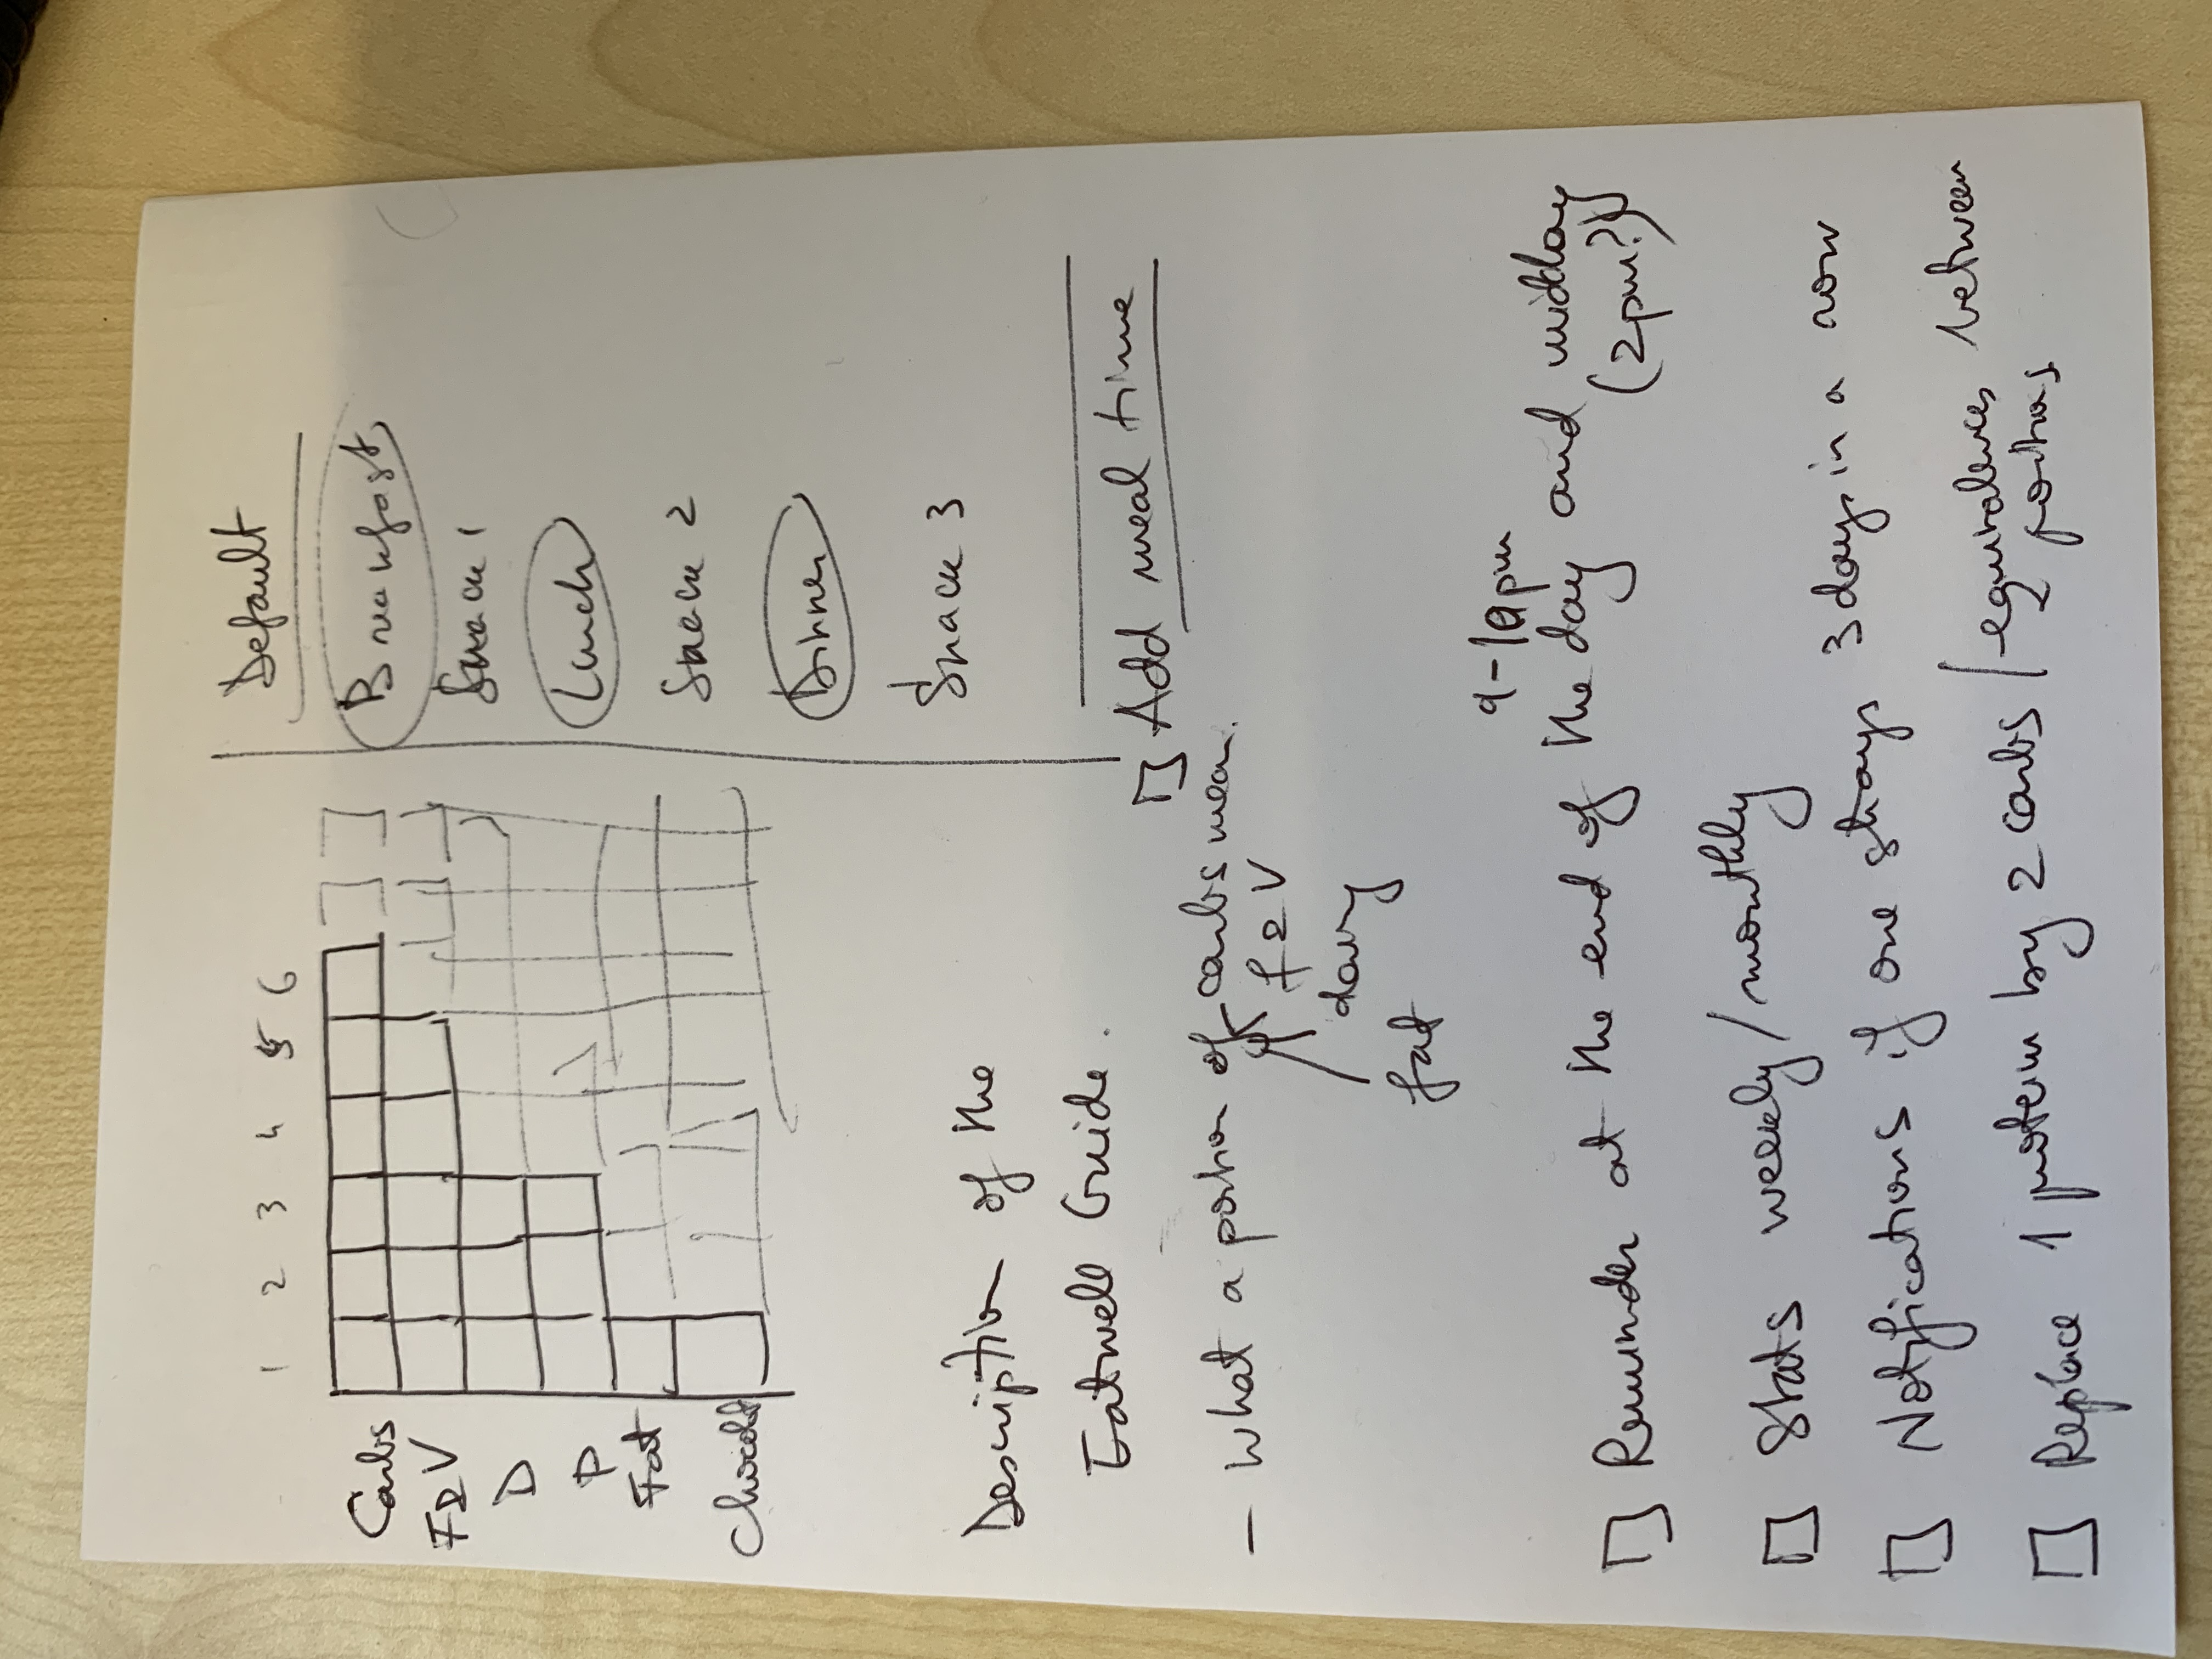
\includegraphics[width=\textwidth,angle=270]{scans/portion0.jpg}
    \caption{Example paper log displayed at first meet}%\label{fig:example_log}
\end{figure}

\begin{figure}
    \centering
    \noindent\begin{subfigure}{.49\textwidth}
    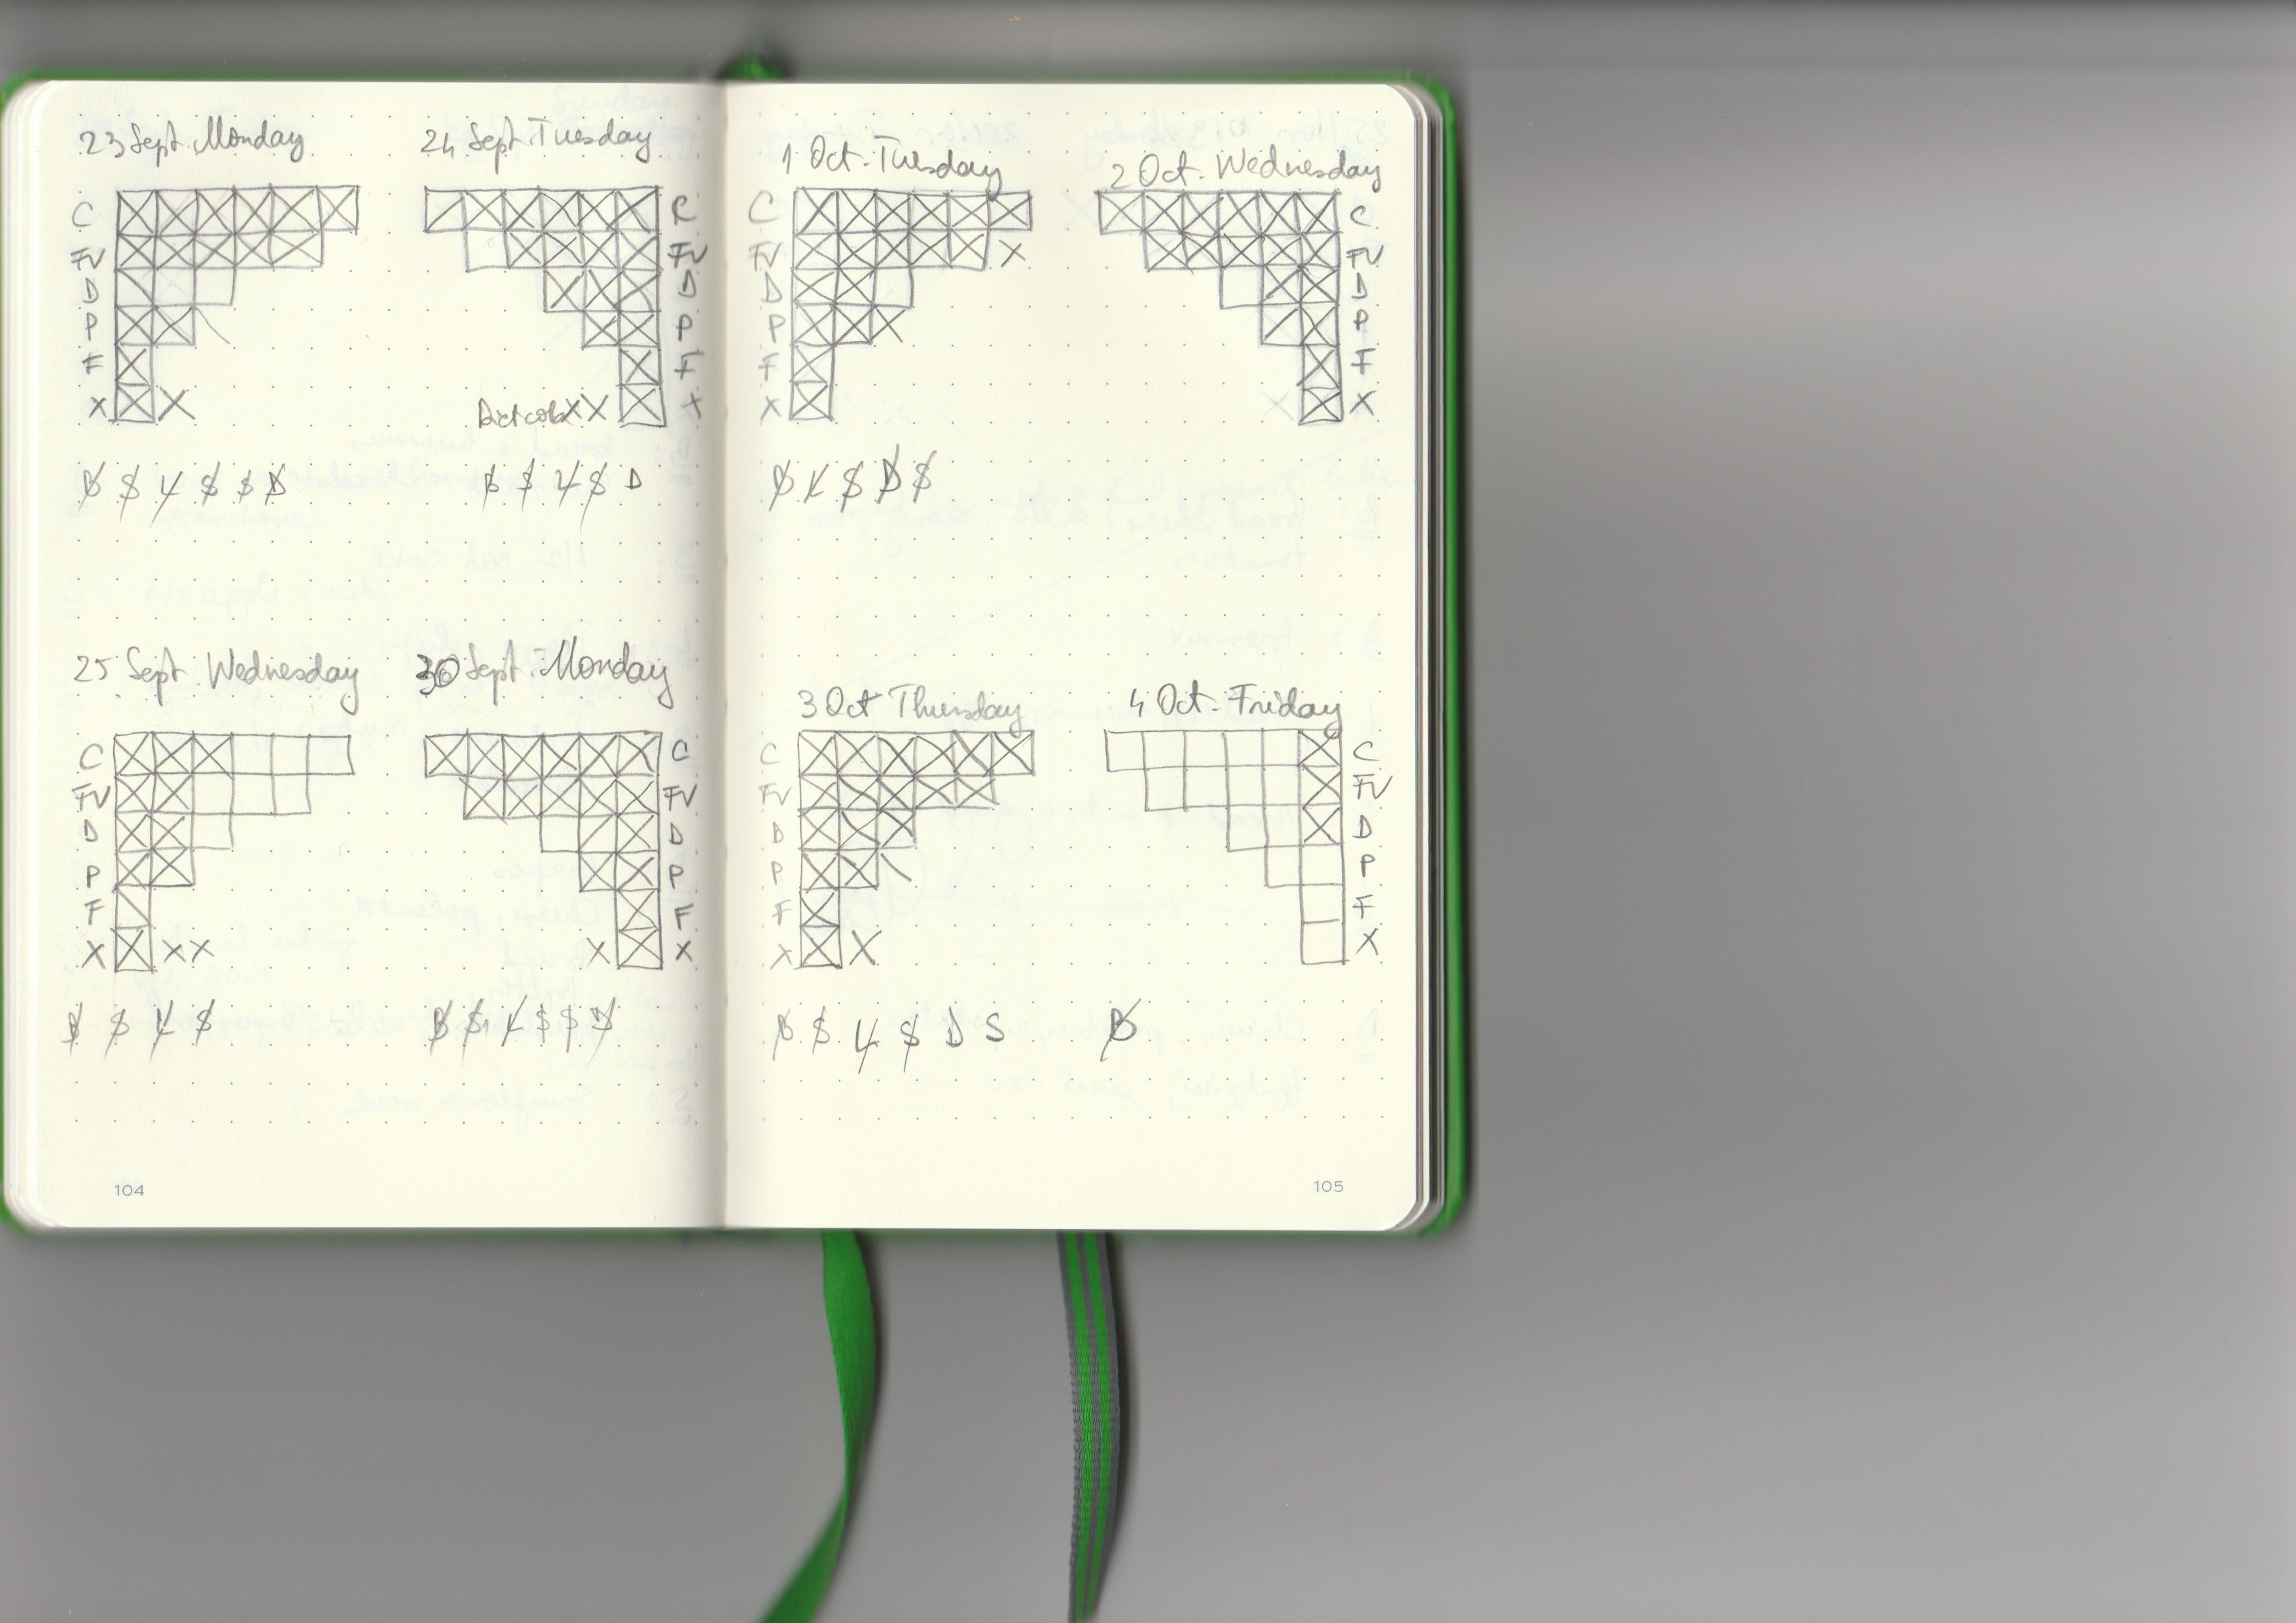
\includegraphics[width=\textwidth,trim={0 20cm 40cm 0},clip]{scans/portion1.jpg}
    \end{subfigure}\hfill
    \begin{subfigure}{.49\textwidth}
    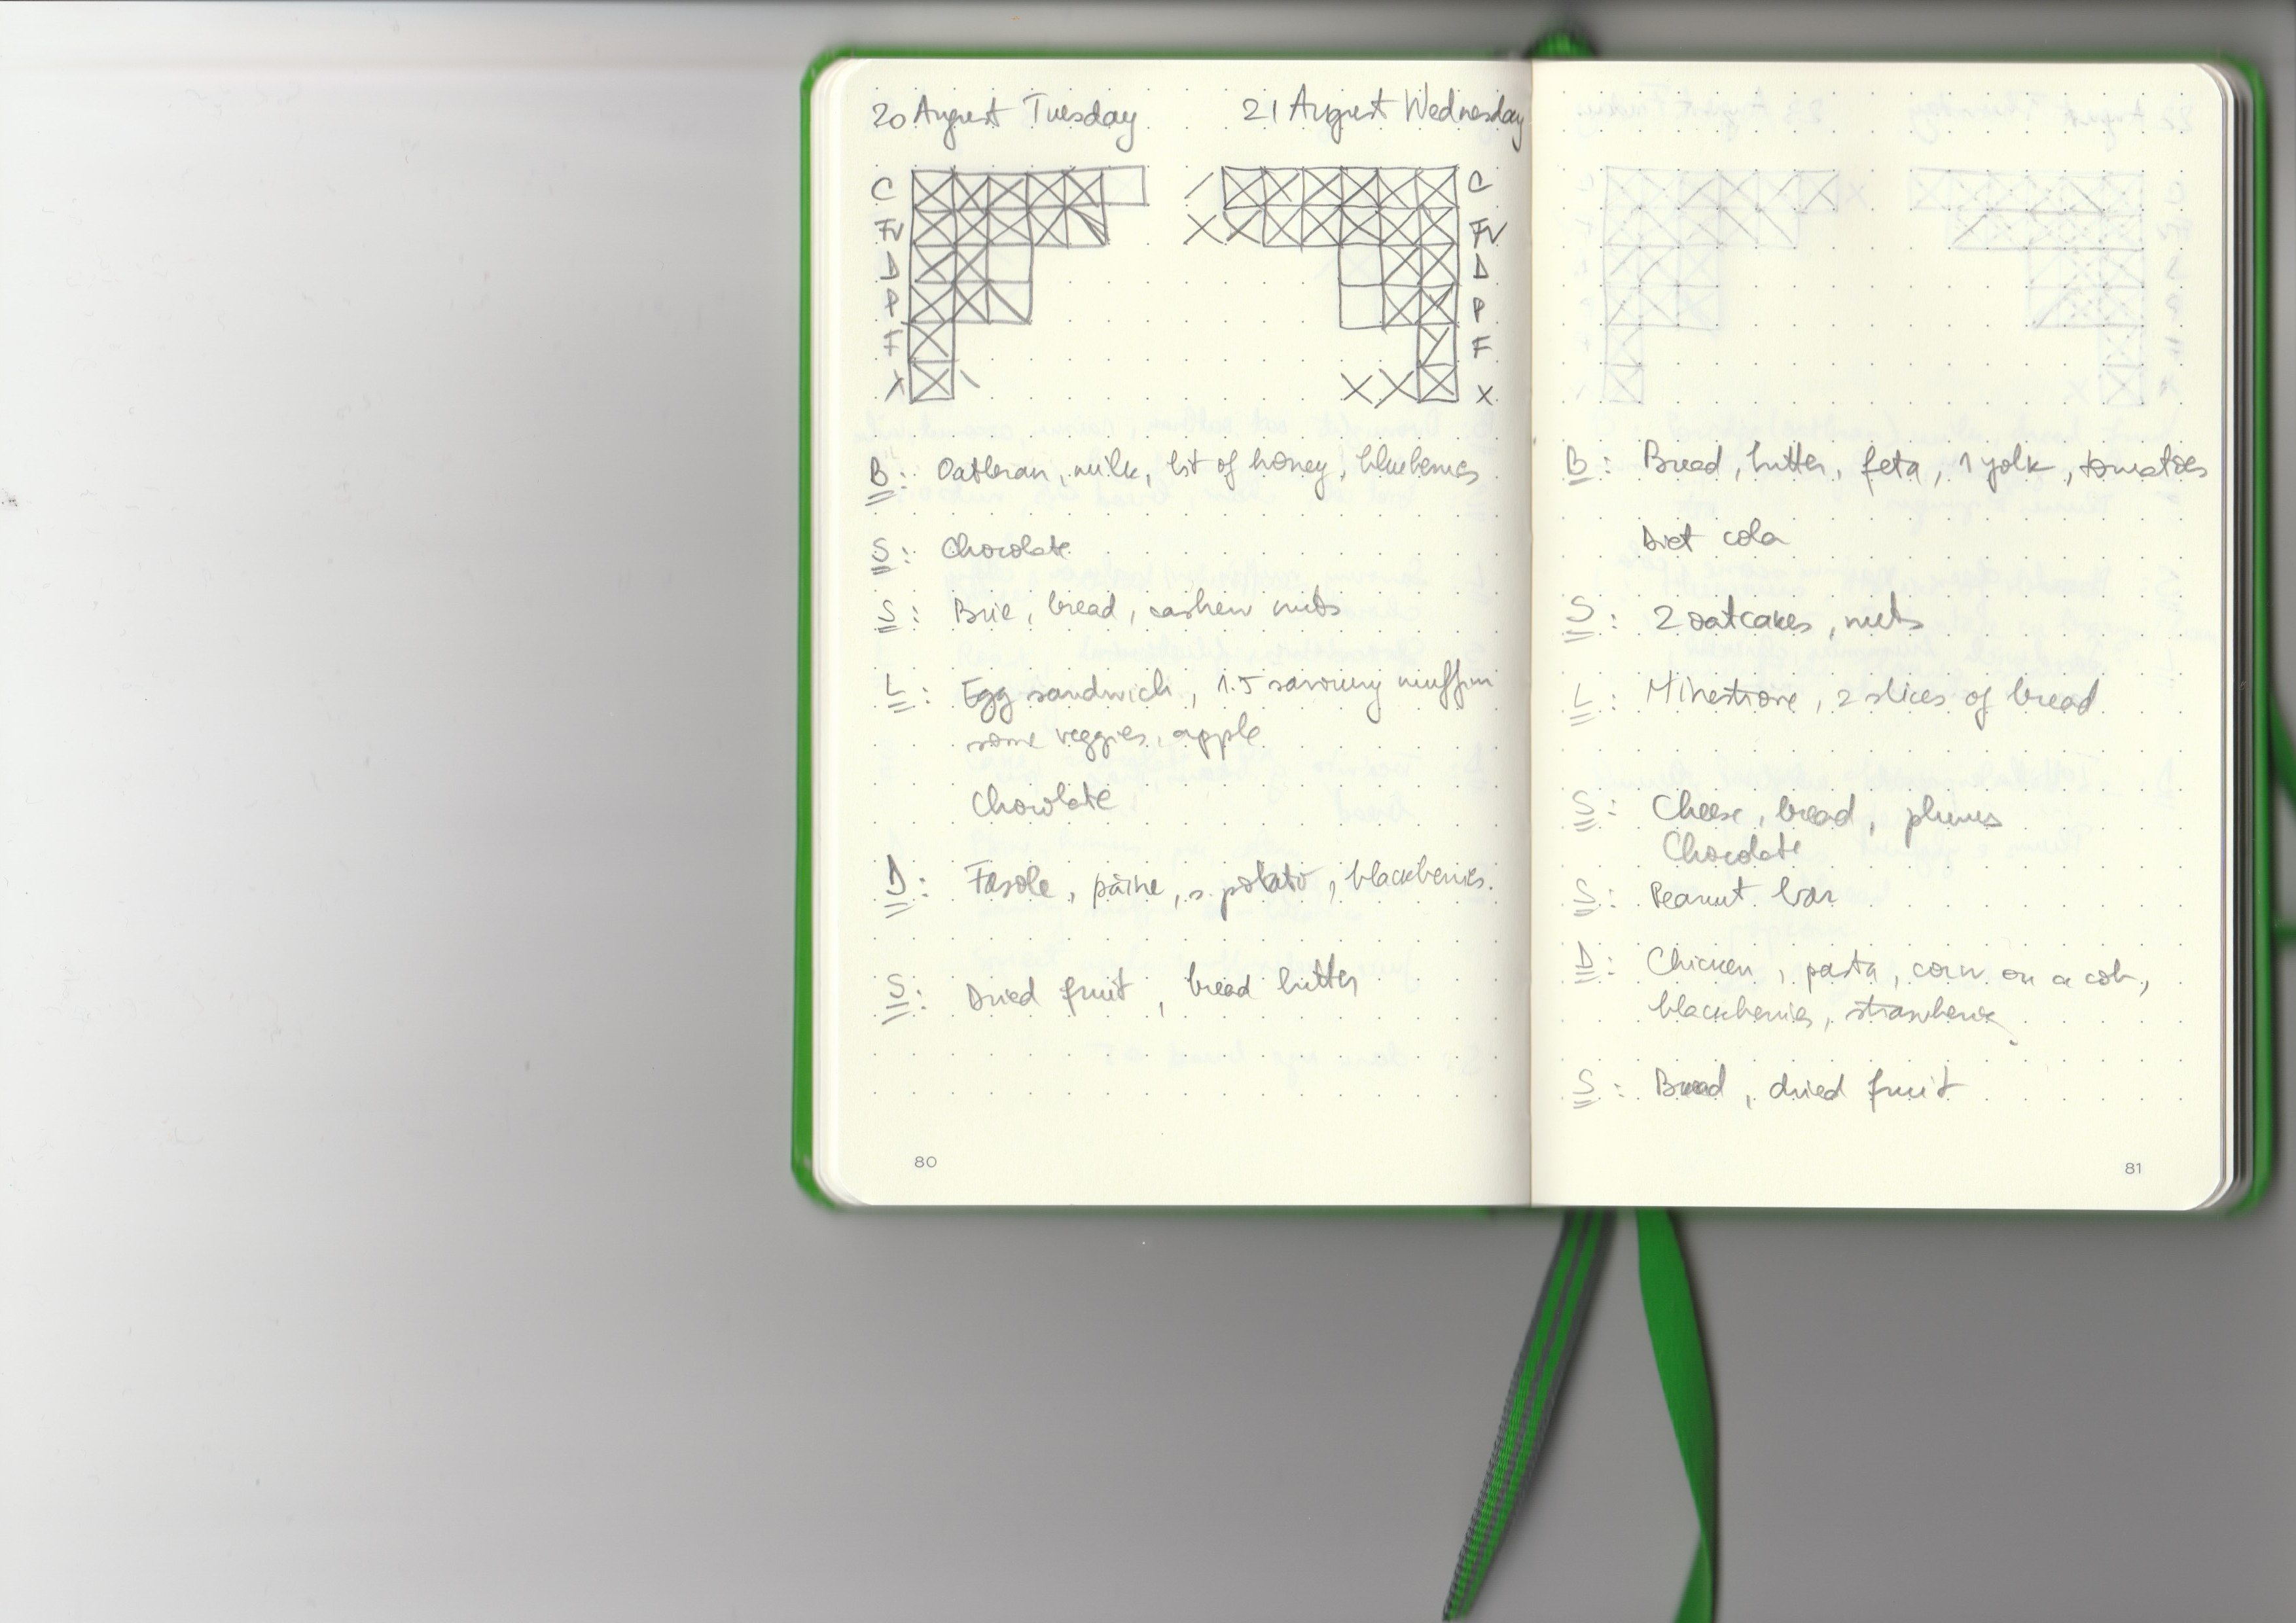
\includegraphics[width=\textwidth,trim={40cm 20cm 0 0},clip]{scans/portion3.jpg}
    \end{subfigure}
    \caption{More scans of practical usage of paper logs}%\label{fig:more_paper_logs}
\end{figure}

\begin{figure}
    \centering
    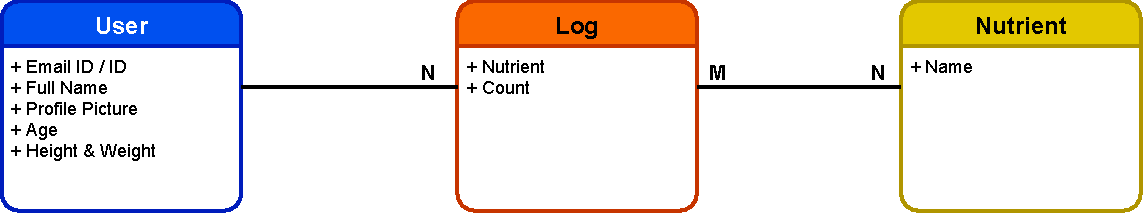
\includegraphics[width=\textwidth]{diagrams/ER_initial.pdf}
    \caption{Initial Entity Relationship model}%\label{fig:ER_initial}
\end{figure}

\begin{figure}
    \centering
    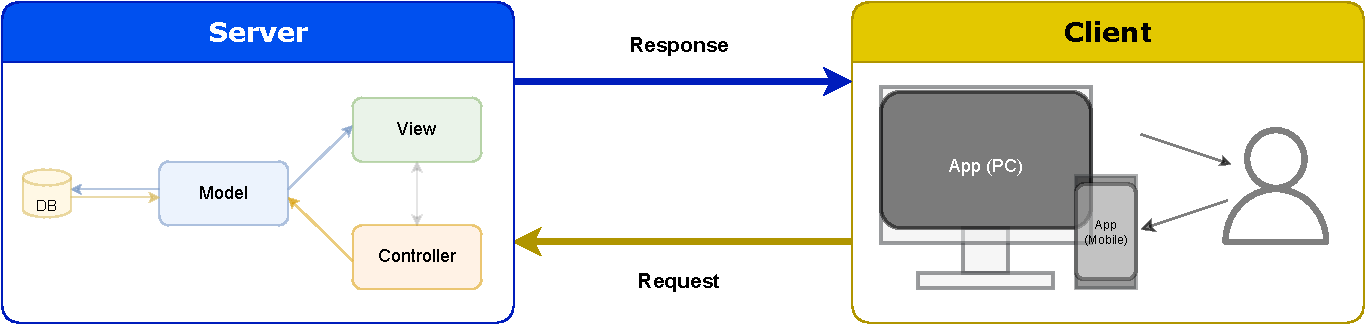
\includegraphics[width=\textwidth]{diagrams/REST.pdf}
    \caption{Overview of REST Architecture}%\label{fig:REST}
\end{figure}

\begin{figure}
    \centering
    \noindent\begin{subfigure}{.48\textwidth}
    \centering
    \frame{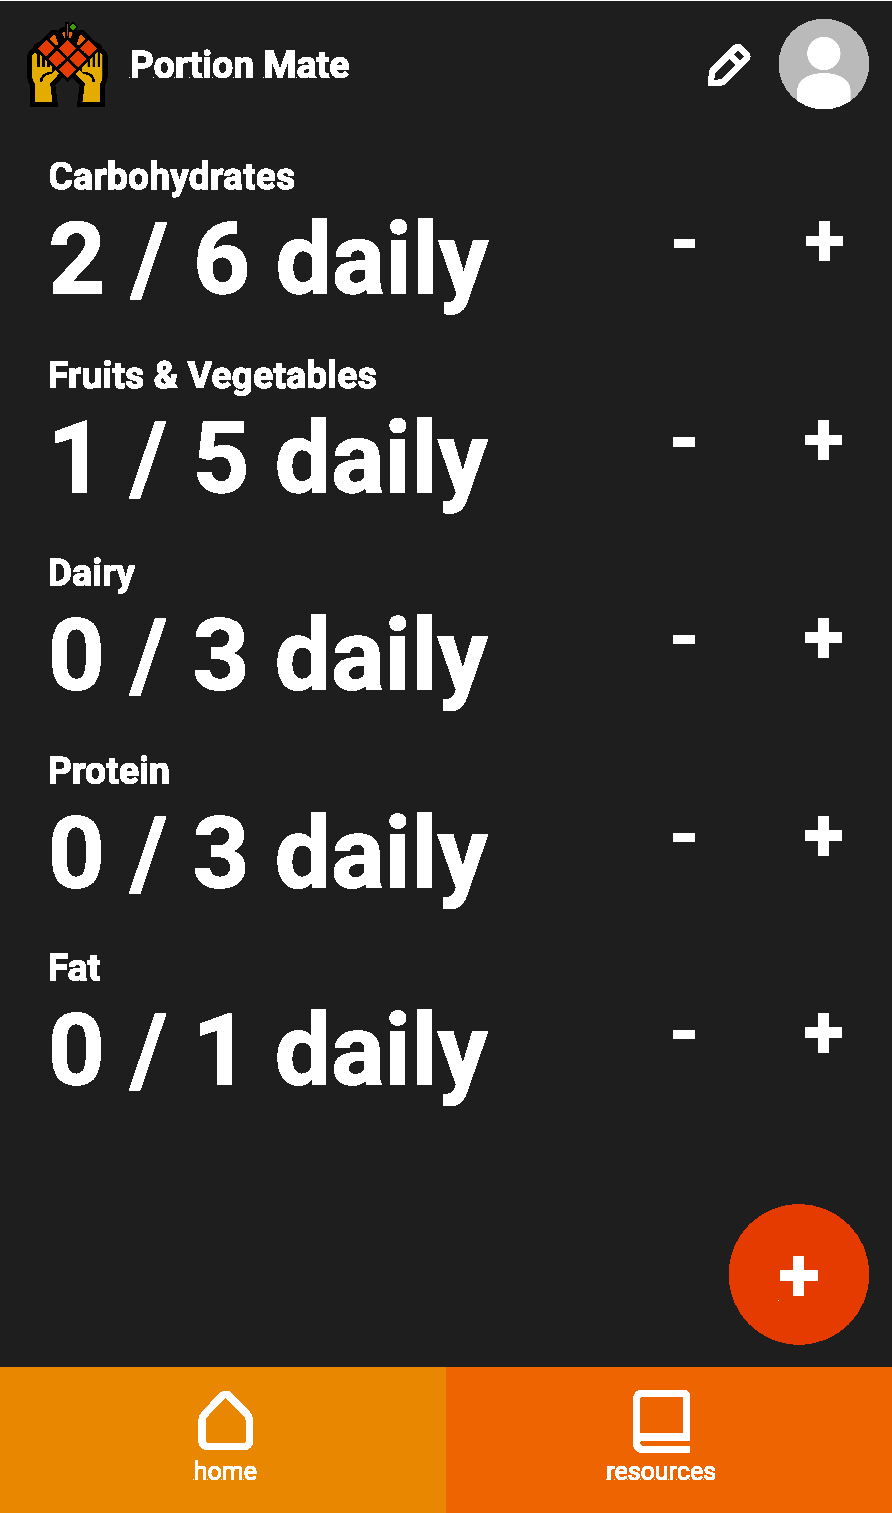
\includegraphics[height=8cm]{wireframes/initial/Fresh Landing [dark].pdf}}
    \caption{Home page}
    \end{subfigure}\hfill
    \begin{subfigure}{.48\textwidth}
    \centering
    \frame{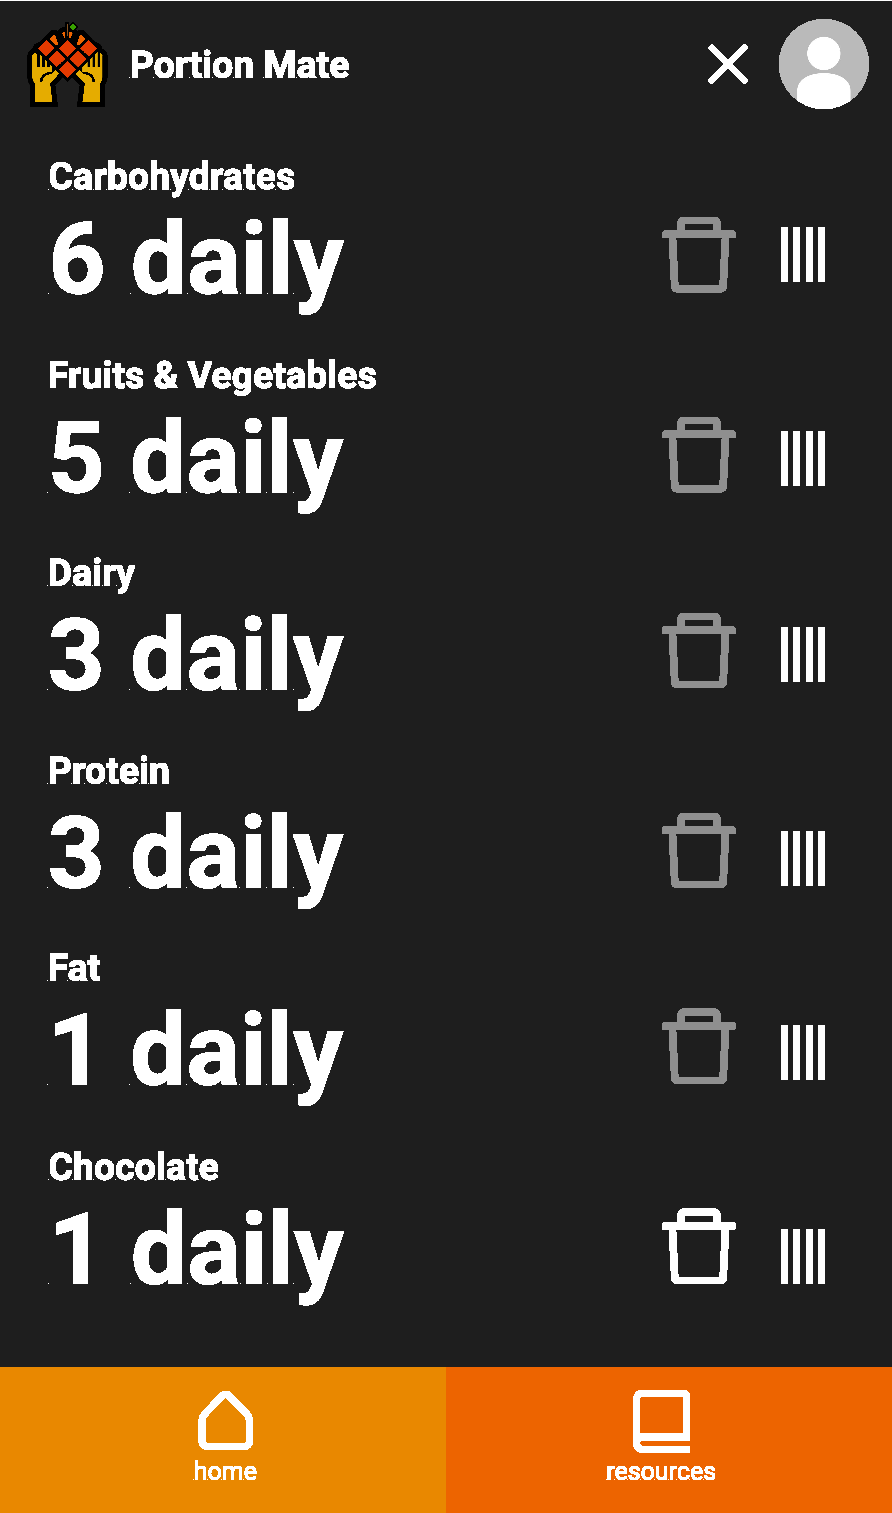
\includegraphics[height=8cm]{wireframes/initial/Edit Landing [dark].pdf}}
    \caption{Edit view of the home page}
    \end{subfigure}
    \caption{Homepage design from initial wireframes}%\label{fig:initial_wireframes}
\end{figure}

\begin{figure}
    \centering
    \noindent\begin{subfigure}{.24\textwidth}
    \centering
    \frame{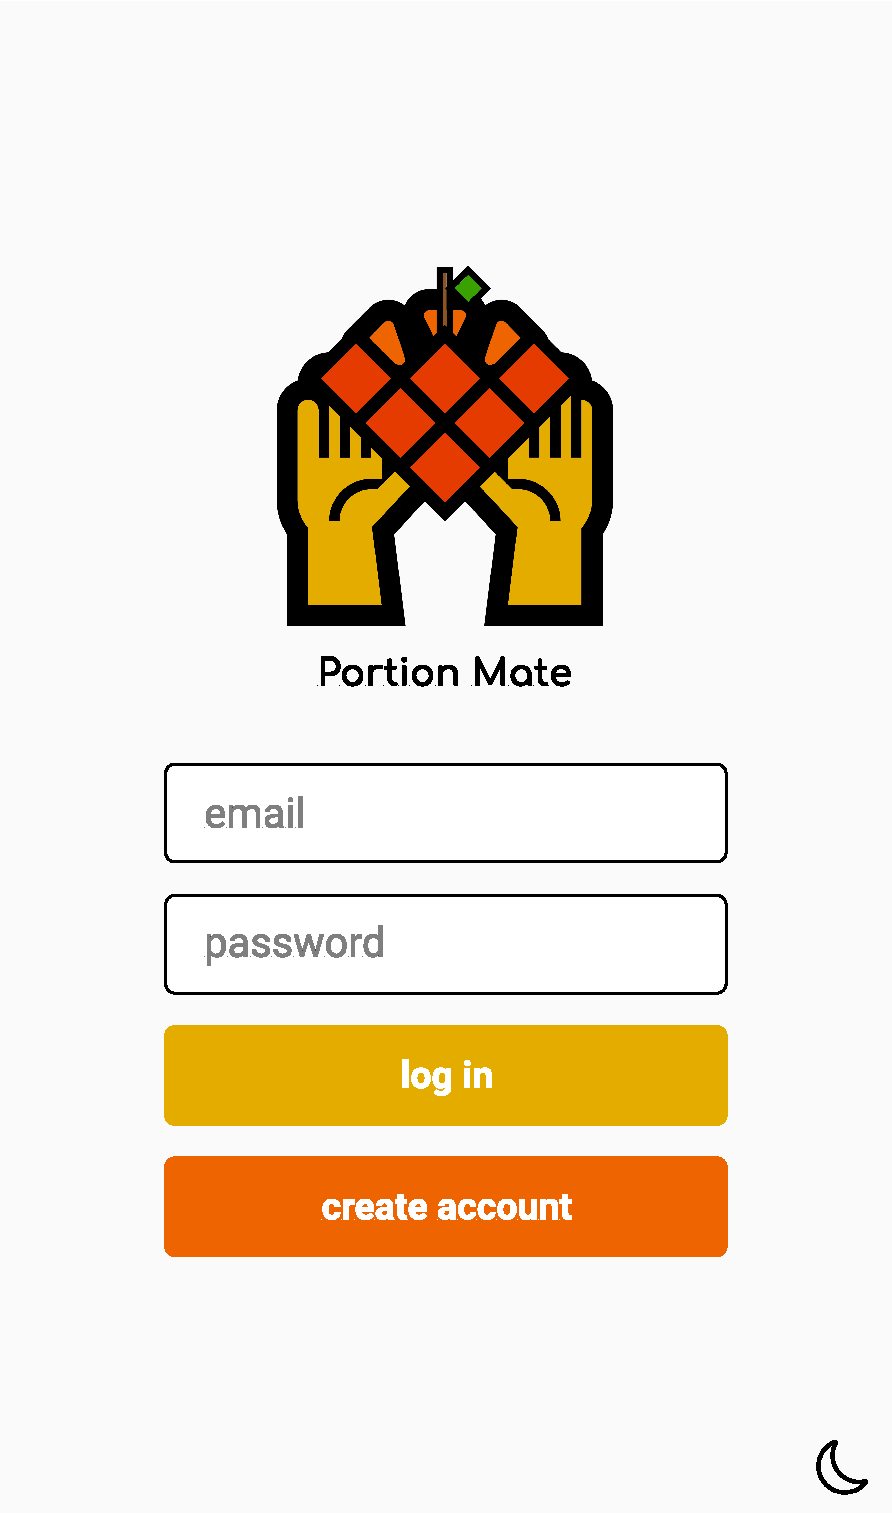
\includegraphics[height=5cm]{wireframes/Login Screen [light].pdf}}
    \caption{Login form (light)}
    \end{subfigure}\hfill
    \begin{subfigure}{.24\textwidth}
    \centering
    \frame{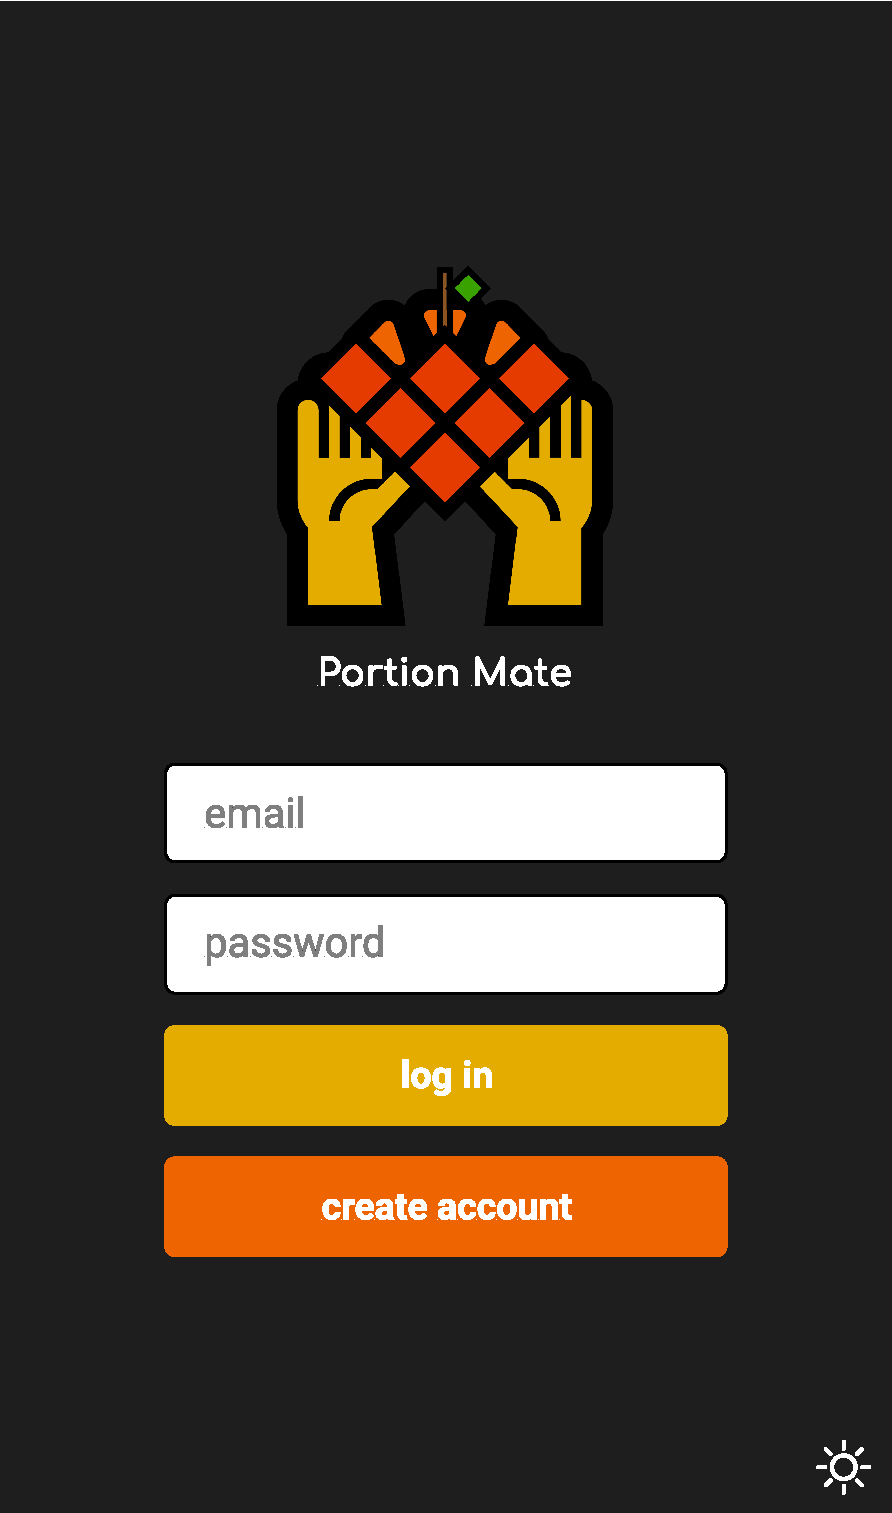
\includegraphics[height=5cm]{wireframes/Login Screen [dark].pdf}}
    \caption{Login form (dark)}
    \end{subfigure}\hfill
    \begin{subfigure}{.24\textwidth}
    \centering
    \frame{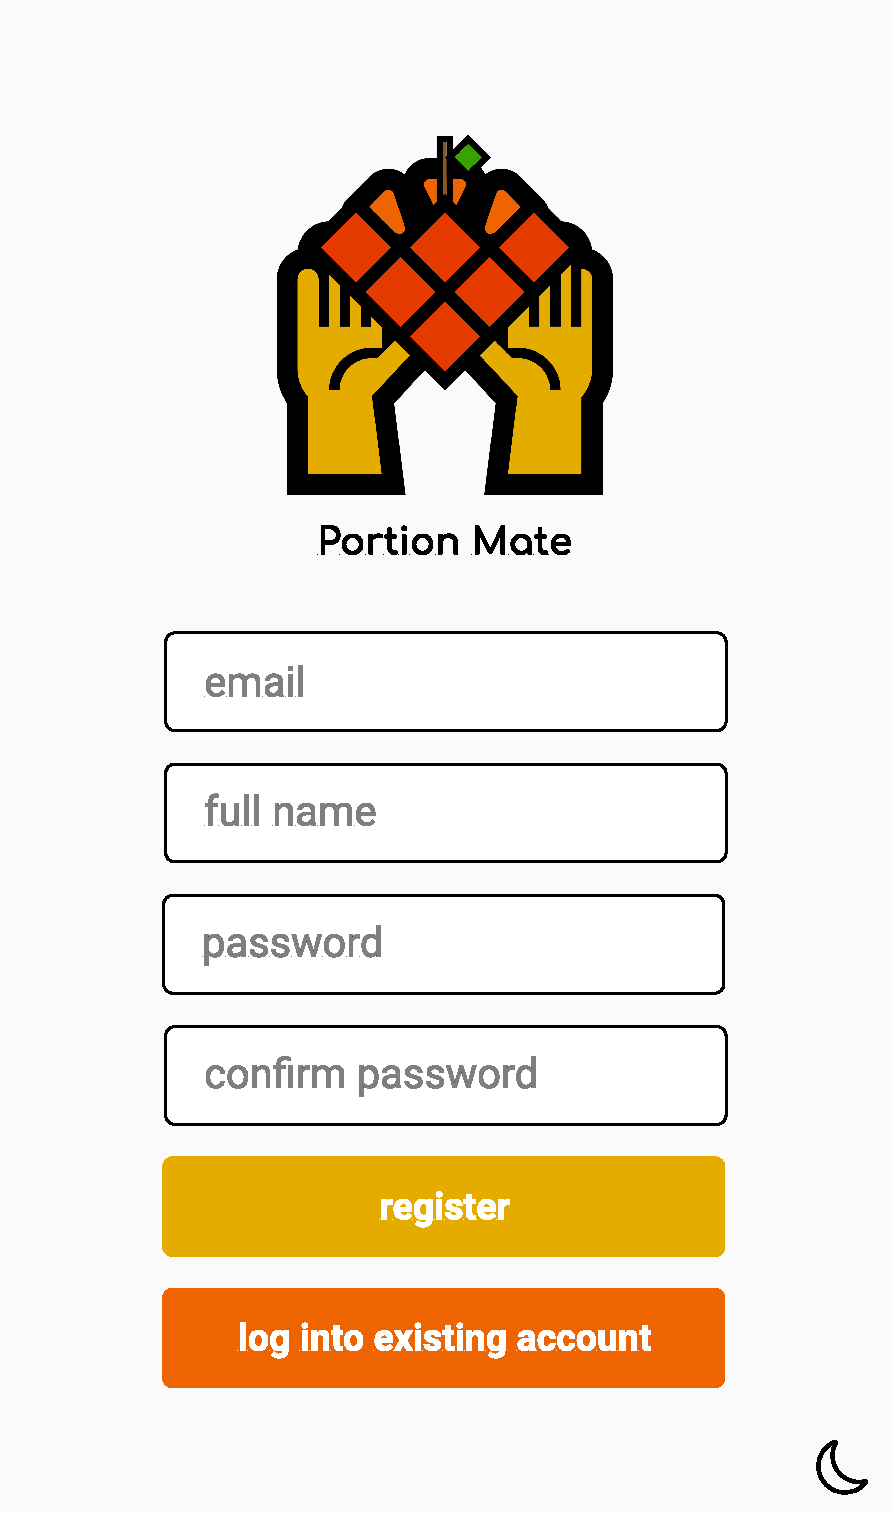
\includegraphics[height=5cm]{wireframes/Register Screen [light].pdf}}
    \caption{Register form (light)}
    \end{subfigure}\hfill
    \begin{subfigure}{.24\textwidth}
    \centering
    \frame{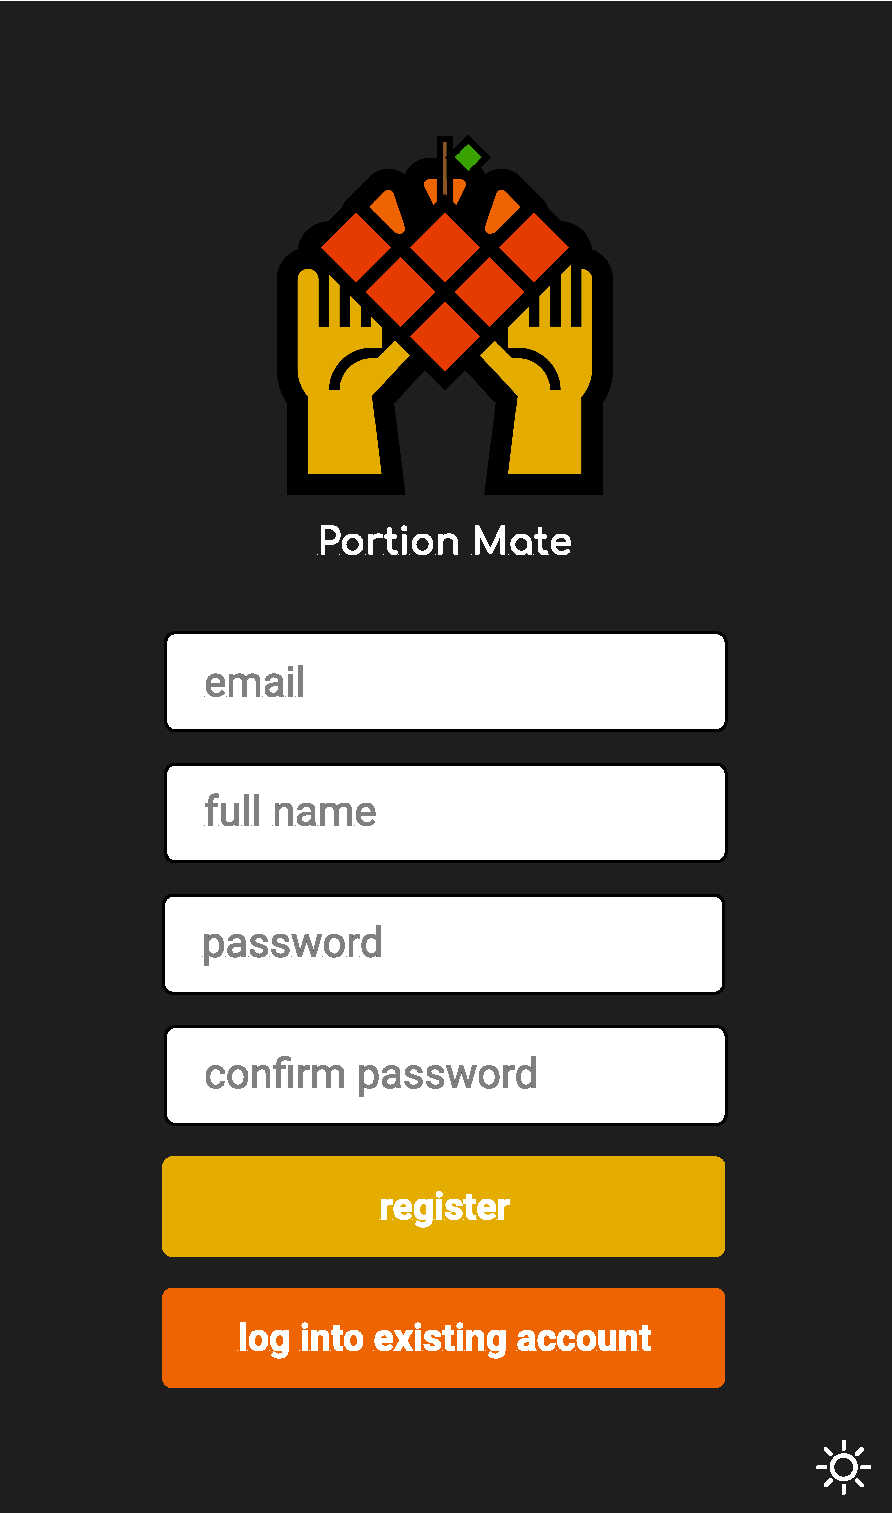
\includegraphics[height=5cm]{wireframes/Register Screen [dark].pdf}}
    \caption{Register form (dark)}
    \end{subfigure}
    \vskip\baselineskip
    \noindent\begin{subfigure}{.24\textwidth}
    \centering
    \frame{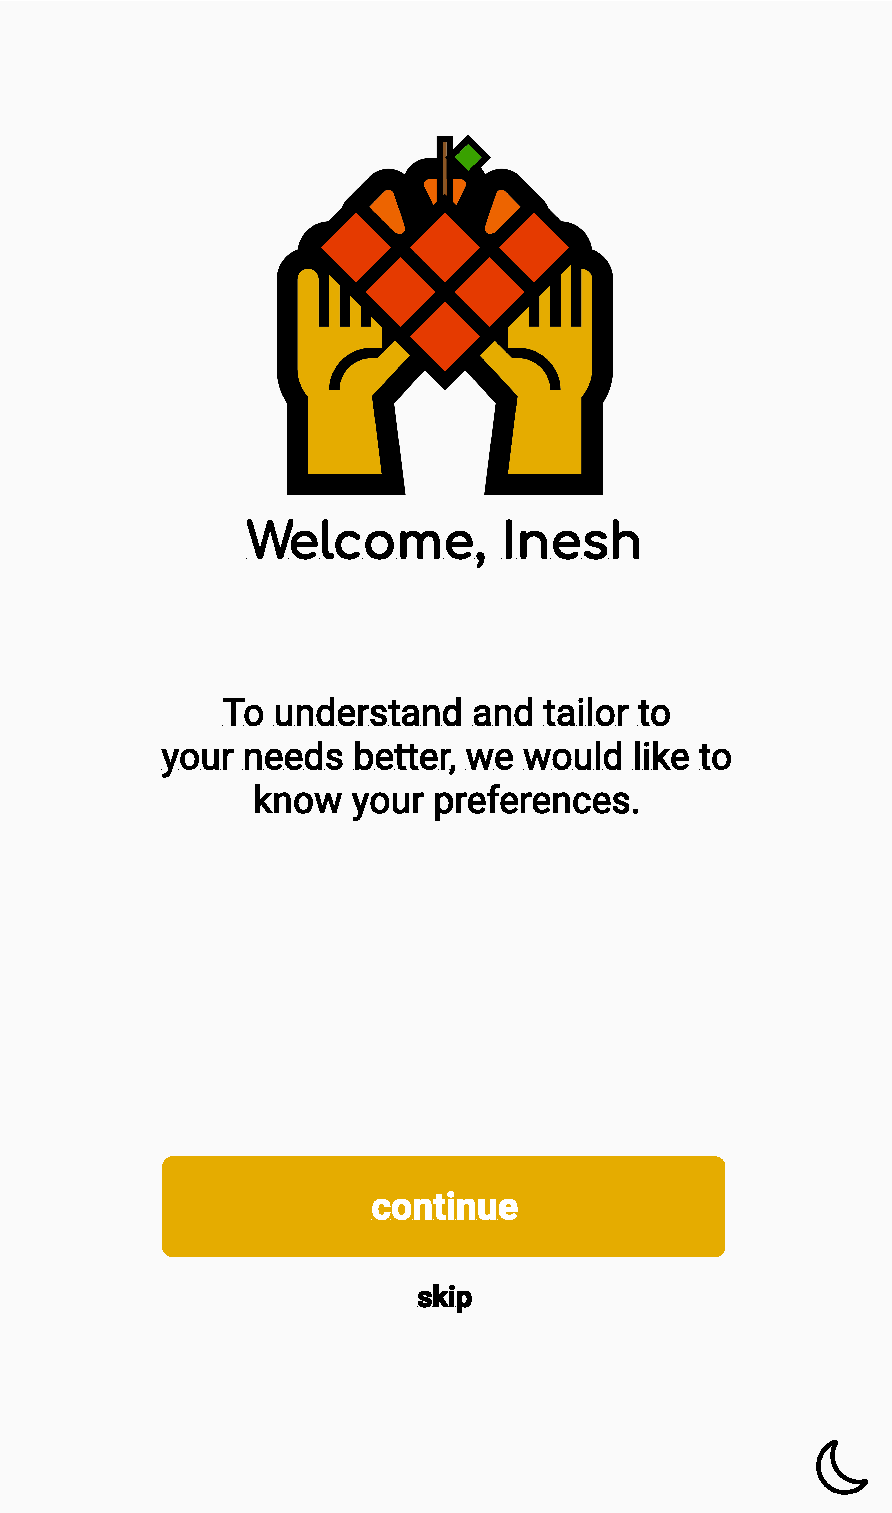
\includegraphics[height=5cm]{wireframes/Registration Welcome Questionnaire - 1 [light].pdf}}
    \caption{Welcome (light)}
    \end{subfigure}\hfill
    \begin{subfigure}{.24\textwidth}
    \centering
    \frame{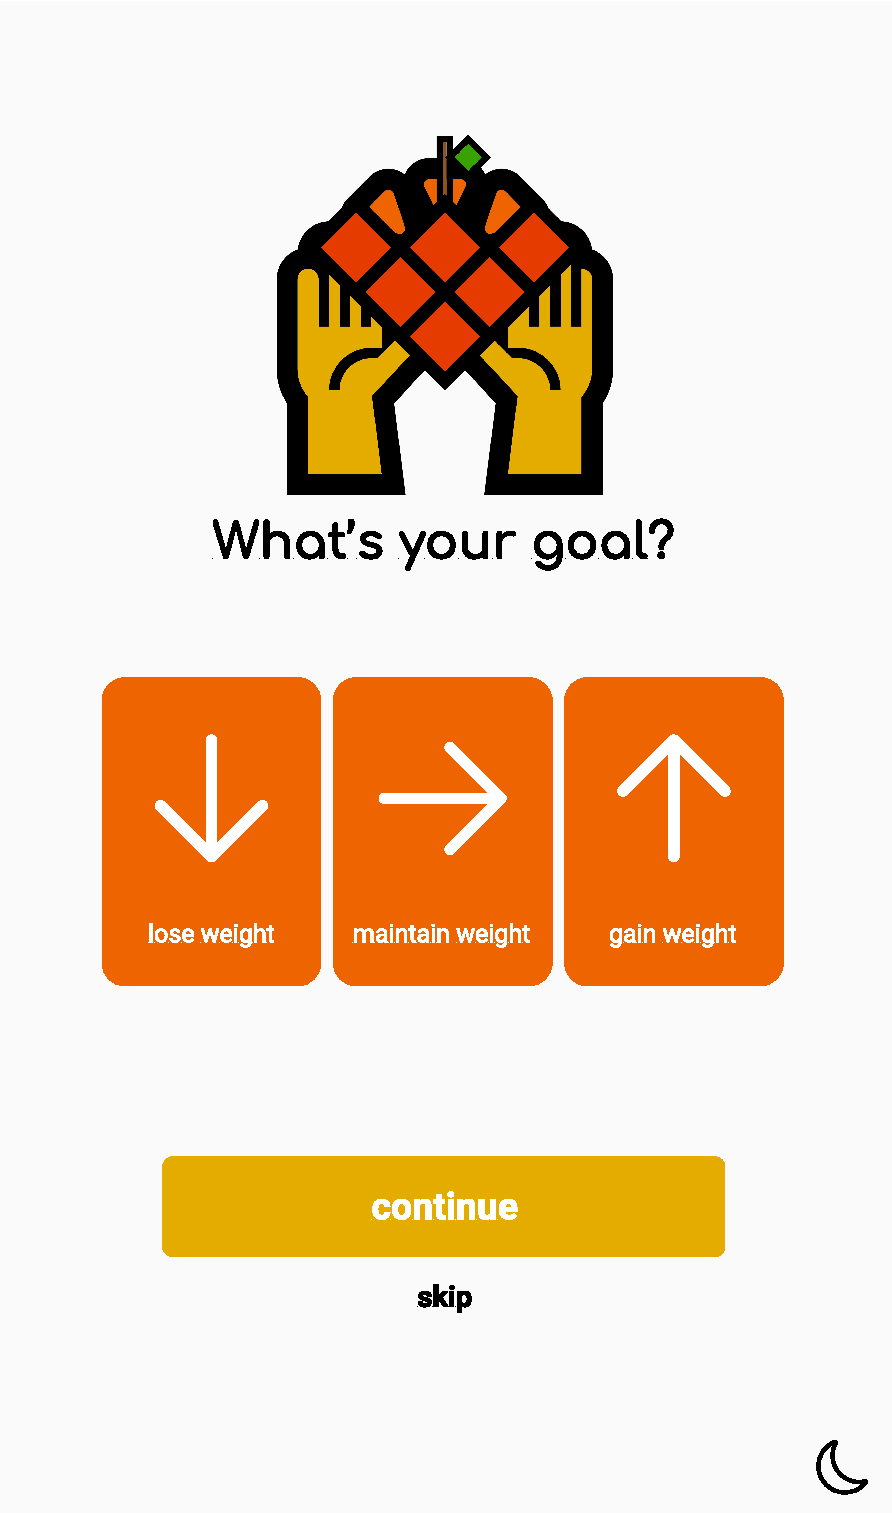
\includegraphics[height=5cm]{wireframes/Registration Welcome Questionnaire - 2 [light].pdf}}
    \caption{Goal inquiry (light)}
    \end{subfigure}\hfill
    \begin{subfigure}{.24\textwidth}
    \centering
    \frame{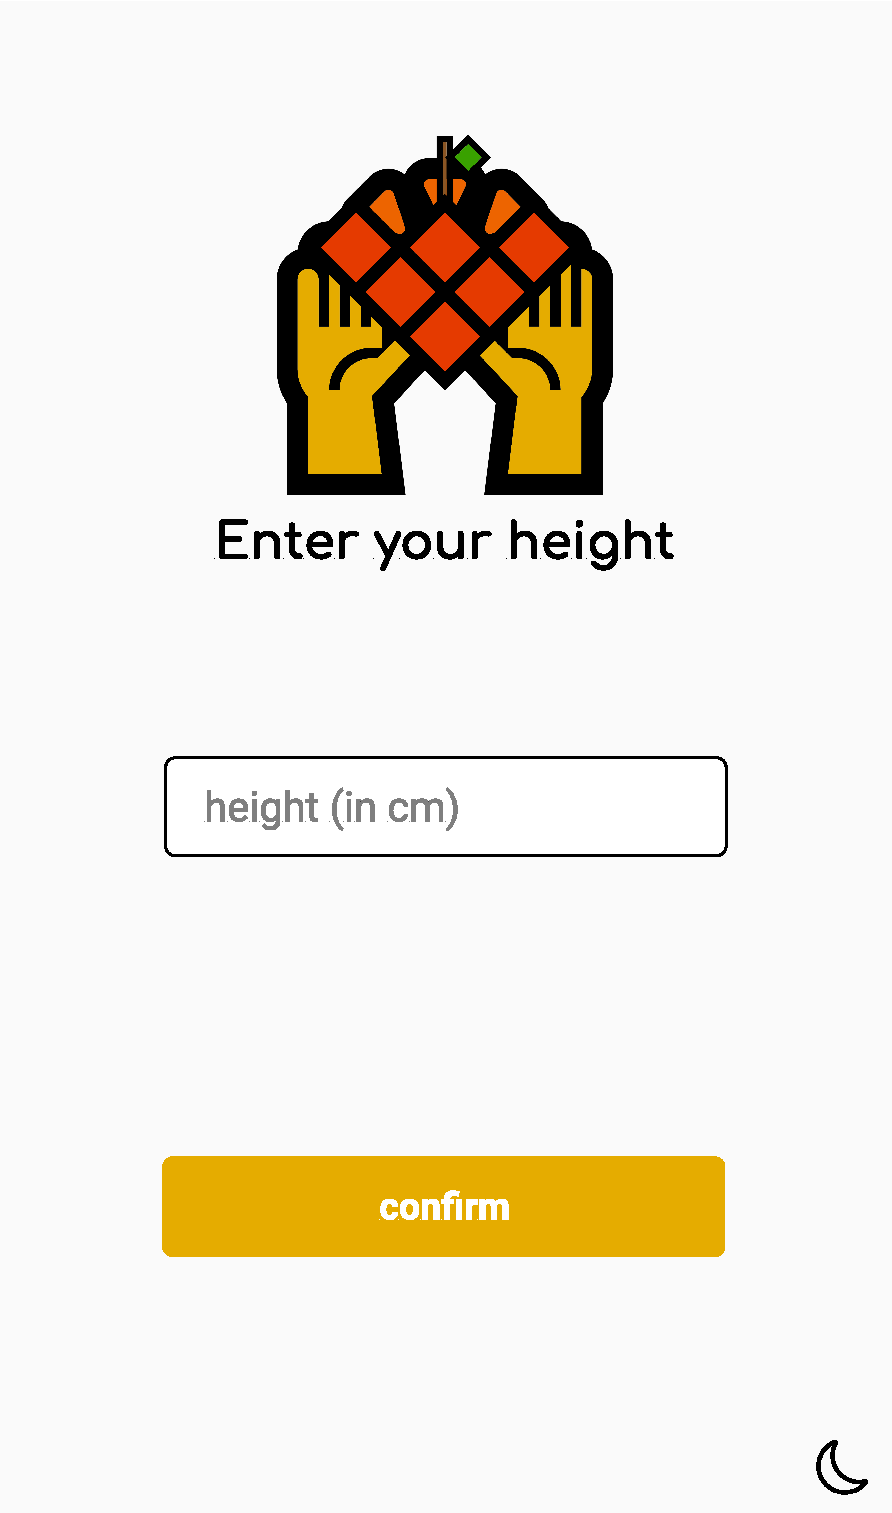
\includegraphics[height=5cm]{wireframes/Registration Welcome Questionnaire - 3 [light].pdf}}
    \caption{Height inquiry (light)}
    \end{subfigure}\hfill
    \begin{subfigure}{.24\textwidth}
    \centering
    \frame{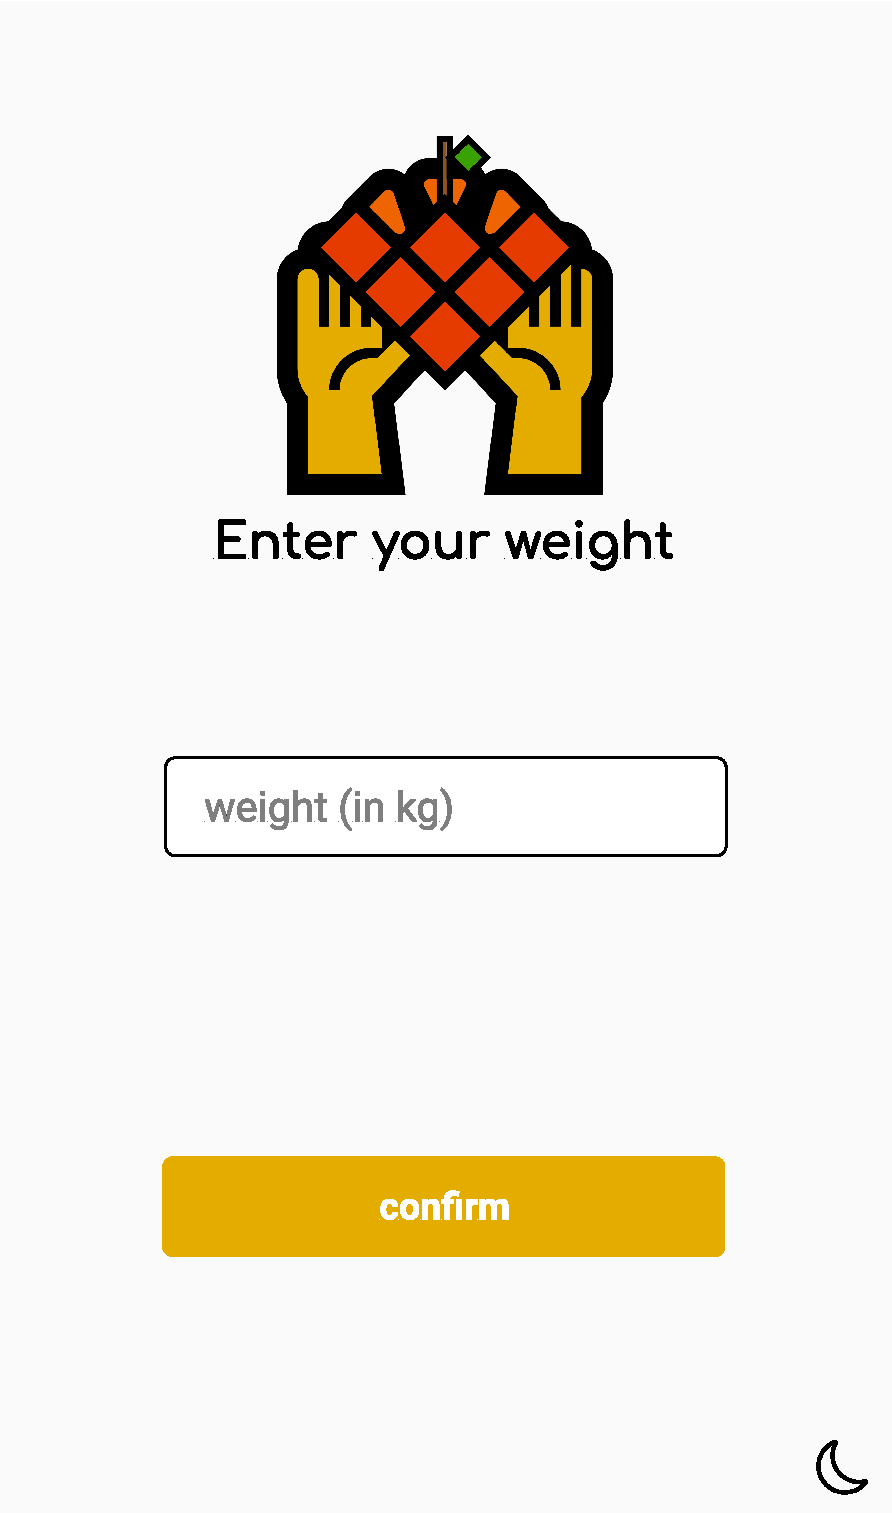
\includegraphics[height=5cm]{wireframes/Registration Welcome Questionnaire - 4 [light].pdf}}
    \caption{Weight inquiry (light)}
    \end{subfigure}
    \vskip\baselineskip
    \noindent\begin{subfigure}{.24\textwidth}
    \centering
    \frame{
\includegraphics[height=5cm]{wireframes/Registration Welcome Questionnaire - 1 [dark].pdf}}
    \caption{Welcome (dark)}
    \end{subfigure}\hfill
    \begin{subfigure}{.24\textwidth}
    \centering
    \frame{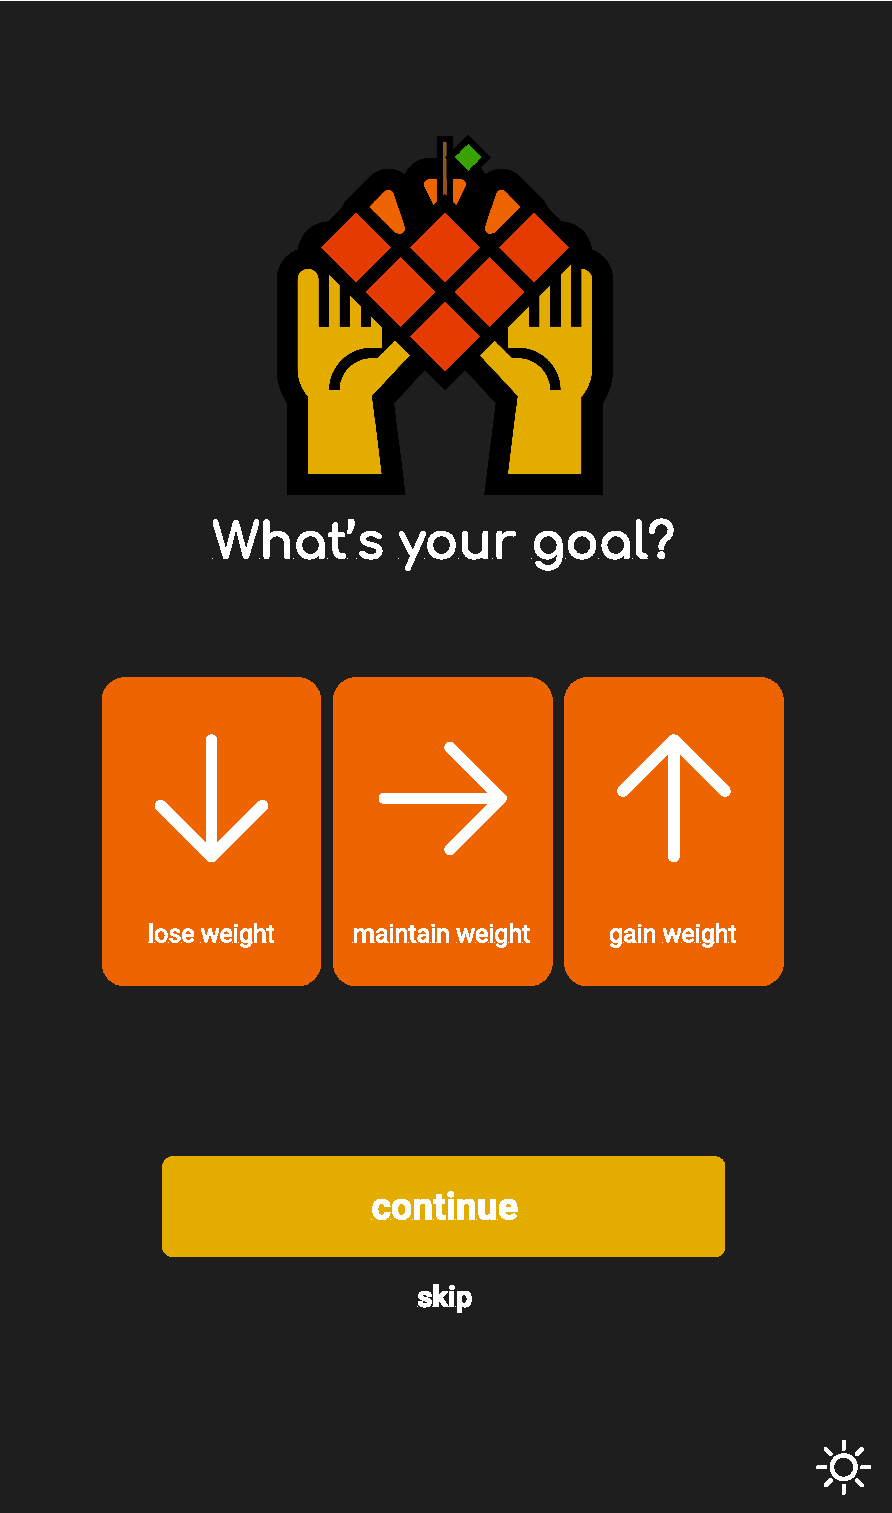
\includegraphics[height=5cm]{wireframes/Registration Welcome Questionnaire - 2 [dark].pdf}}
    \caption{Goal inquiry (dark)}
    \end{subfigure}\hfill
    \begin{subfigure}{.24\textwidth}
    \centering
    \frame{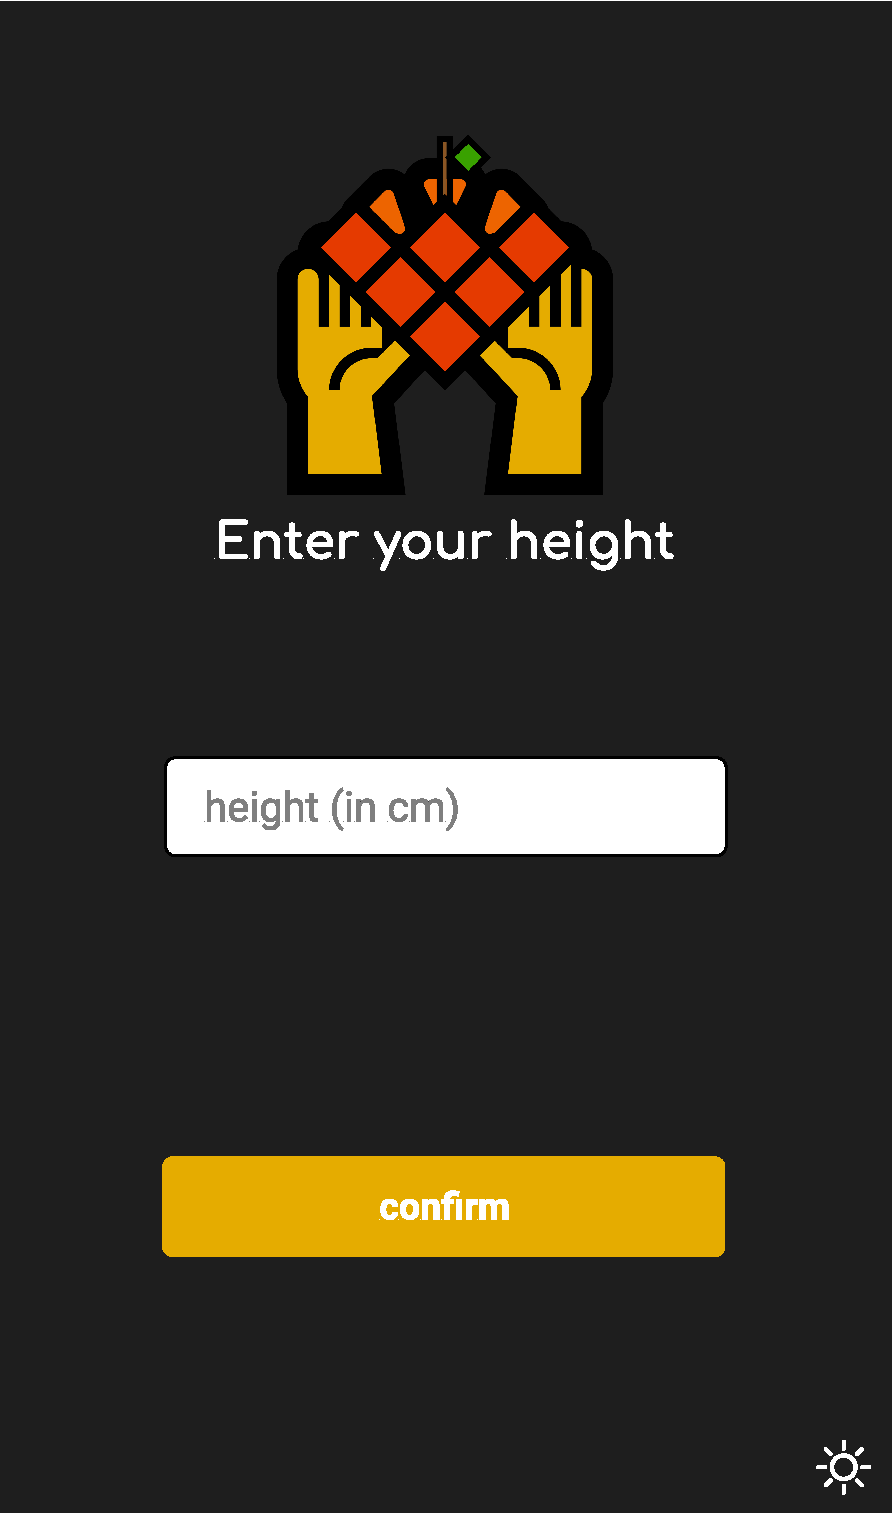
\includegraphics[height=5cm]{wireframes/Registration Welcome Questionnaire - 3 [dark].pdf}}
    \caption{Height inquiry (dark)}
    \end{subfigure}\hfill
    \begin{subfigure}{.24\textwidth}
    \centering
    \frame{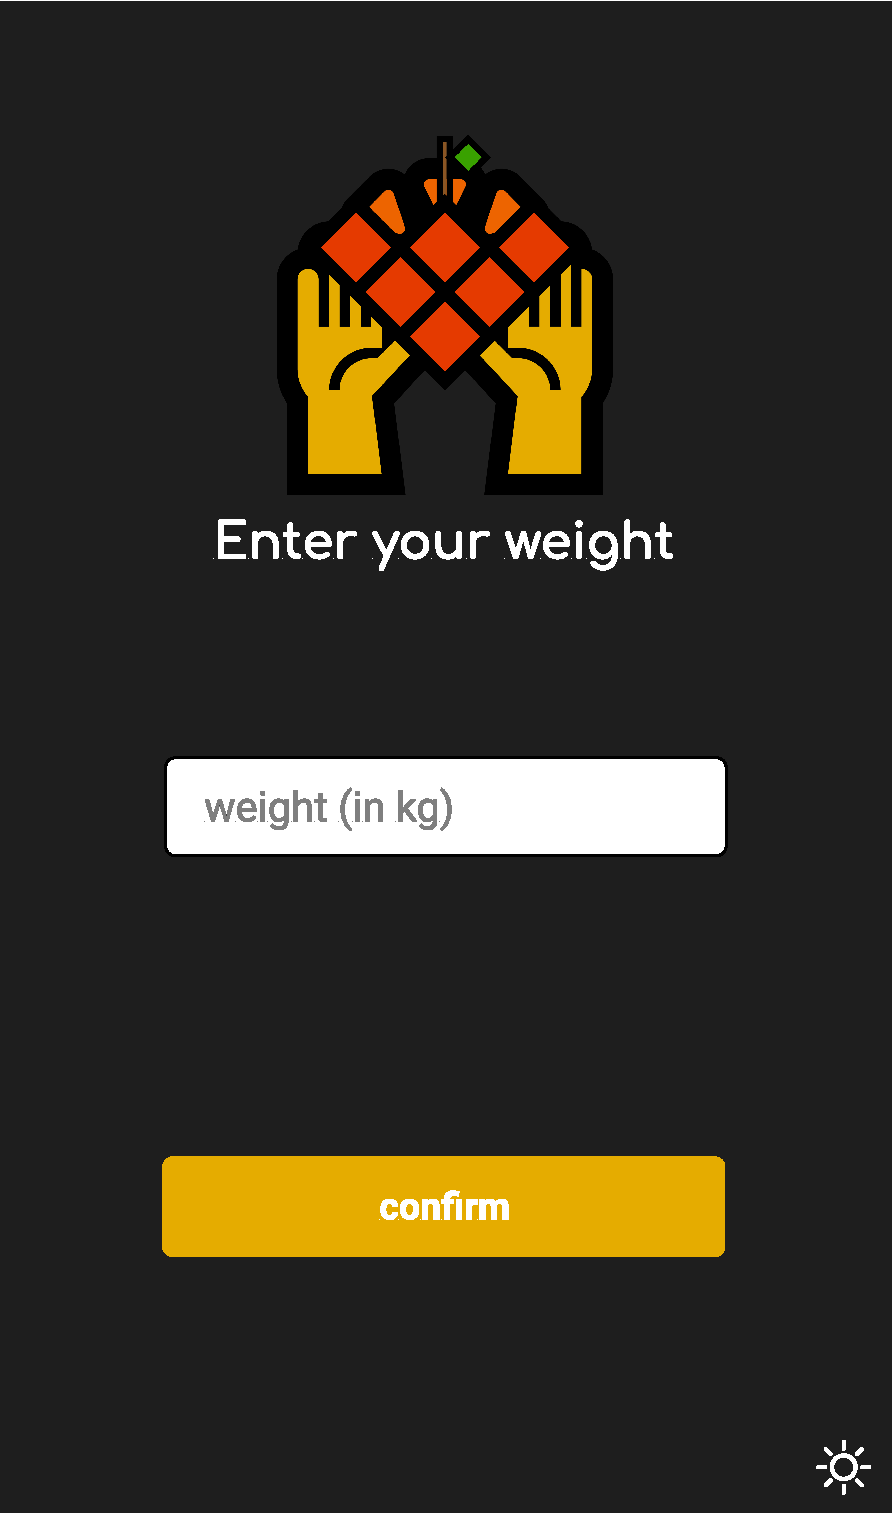
\includegraphics[height=5cm]{wireframes/Registration Welcome Questionnaire - 4 [dark].pdf}}
    \caption{Weight inquiry (dark)}
    \end{subfigure}
    \caption{Wireframes for login and registration}
\end{figure}

\begin{figure}
    \centering
    \noindent\begin{subfigure}{.24\textwidth}
    \centering
    \frame{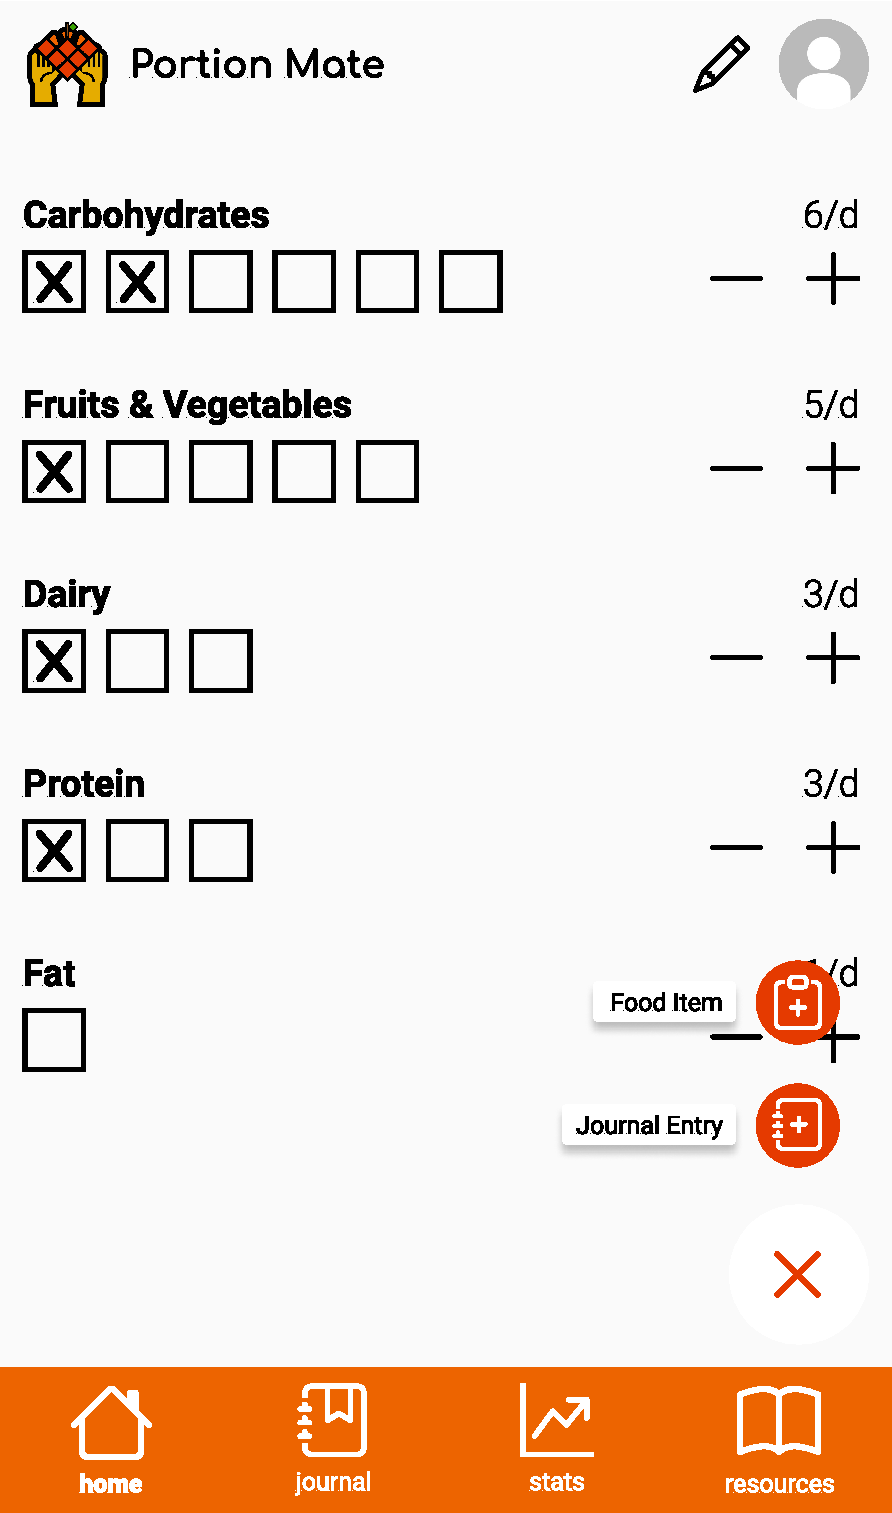
\includegraphics[height=5cm]{wireframes/Landing Action Button Menu [light].pdf}}
    \caption{Home (light)}
    \end{subfigure}\hfill
    \begin{subfigure}{.24\textwidth}
    \centering
    \frame{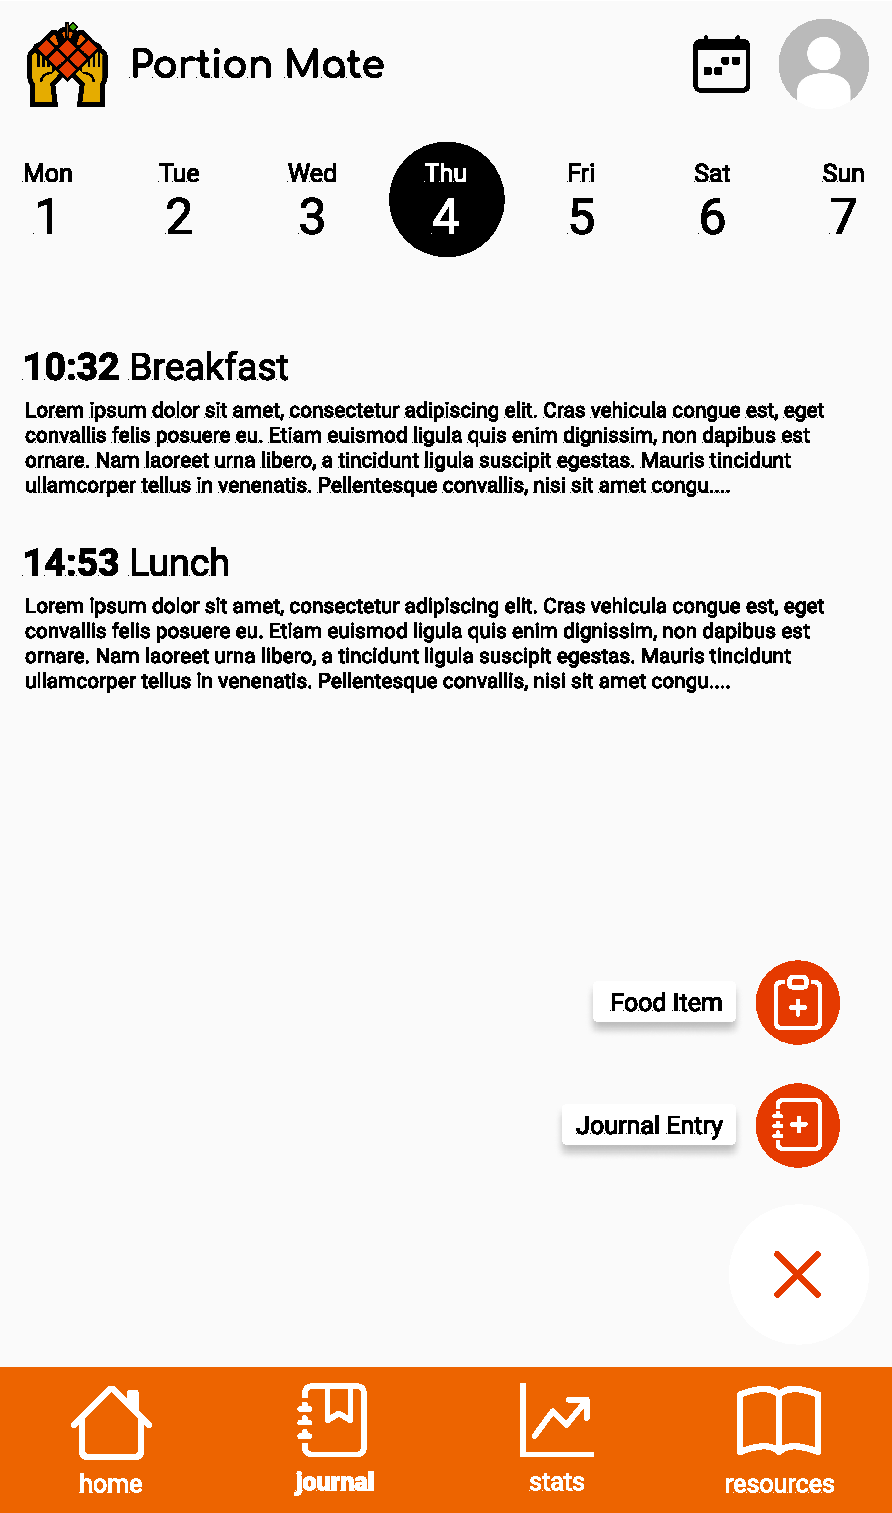
\includegraphics[height=5cm]{wireframes/Journal Action Button Menu [light].pdf}}
    \caption{Journal (light)}
    \end{subfigure}\hfill
    \begin{subfigure}{.24\textwidth}
    \centering
    \frame{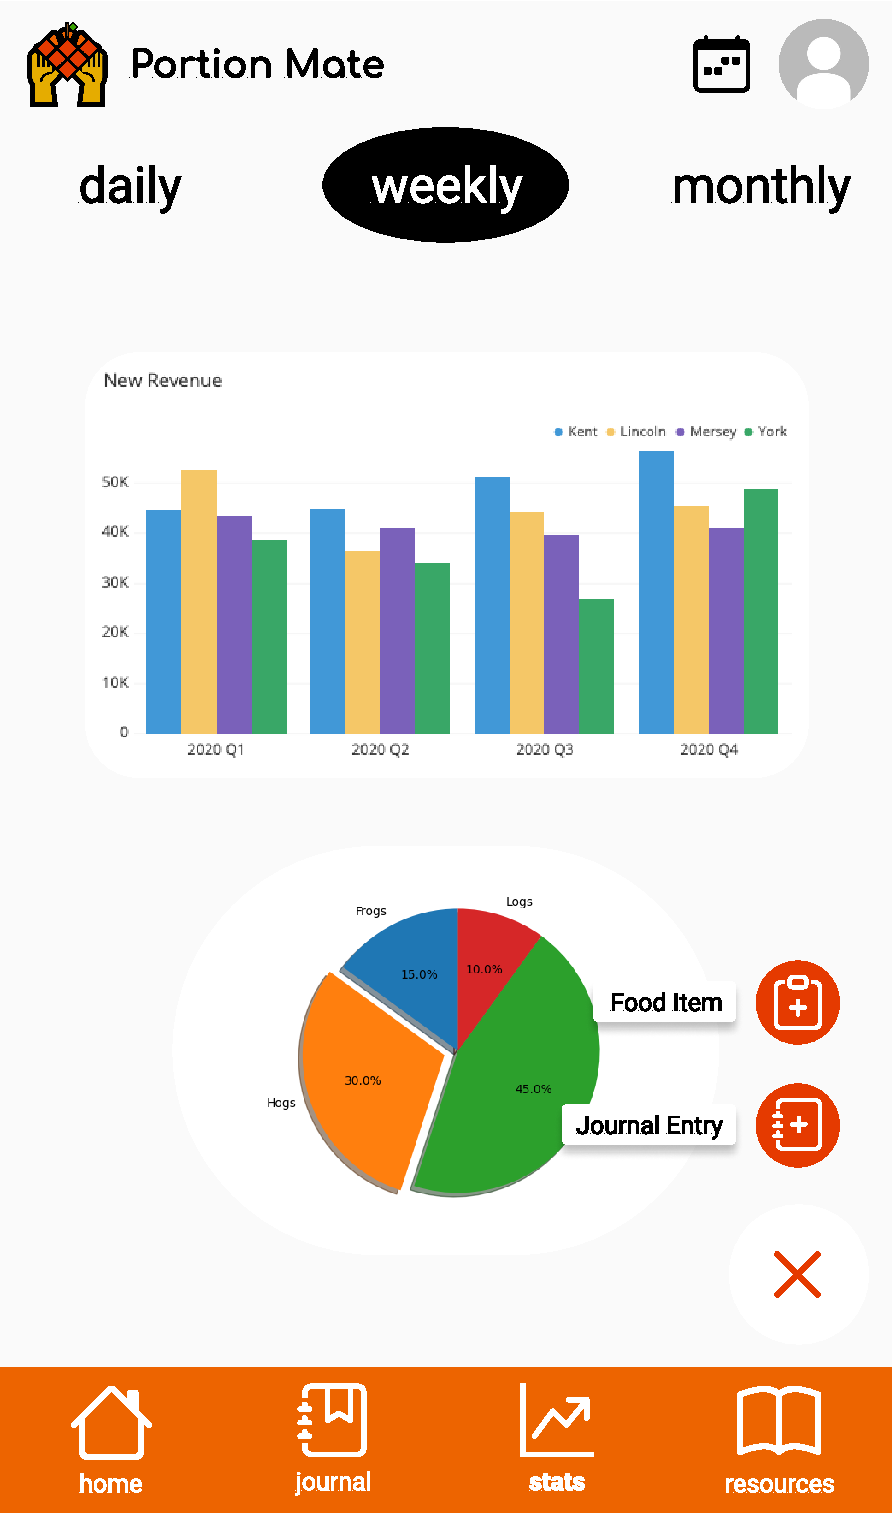
\includegraphics[height=5cm]{wireframes/Stats Action Button Menu [light].pdf}}
    \caption{Stats (light)}
    \end{subfigure}\hfill
    \begin{subfigure}{.24\textwidth}
    \centering
    \frame{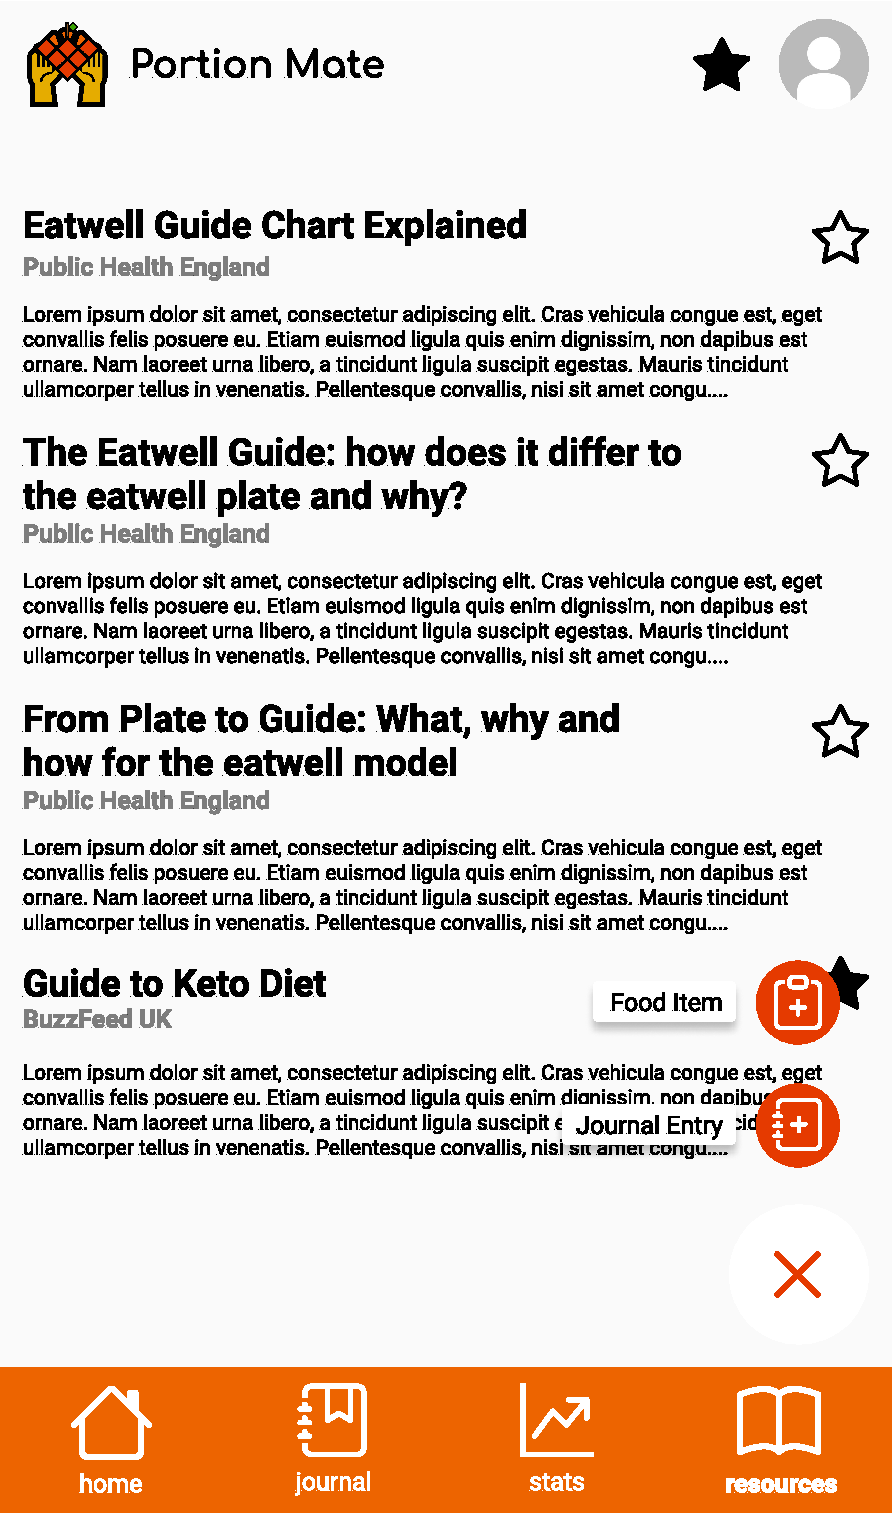
\includegraphics[height=5cm]{wireframes/Resources Action Button Menu [light].pdf}}
    \caption{Resources (light)}
    \end{subfigure}
    \vskip\baselineskip
    \noindent\begin{subfigure}{.24\textwidth}
    \centering
    \frame{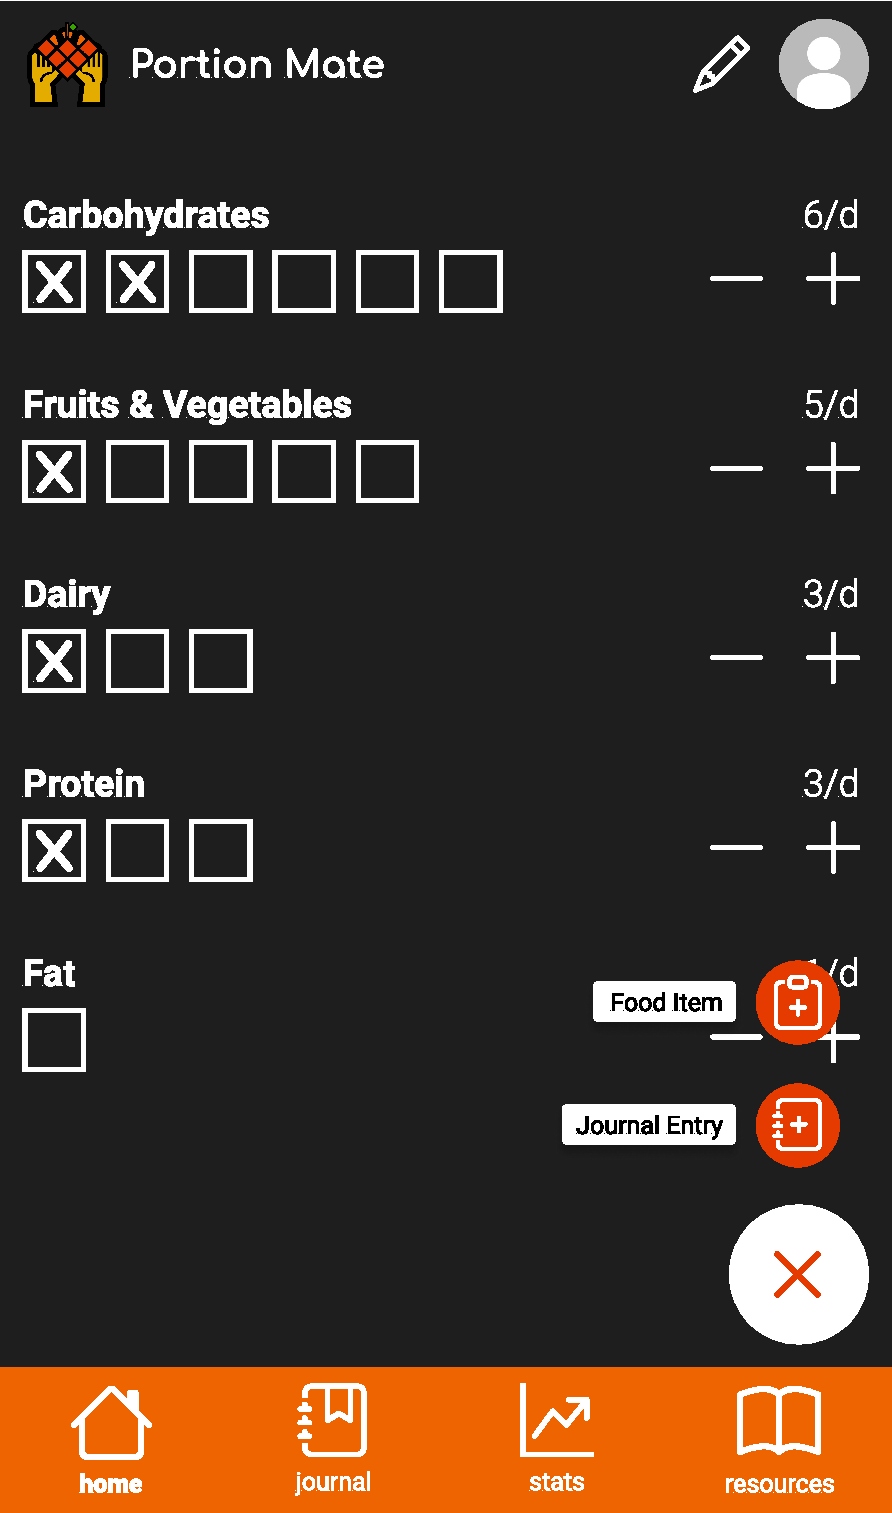
\includegraphics[height=5cm]{wireframes/Landing Action Button Menu [dark].pdf}}
    \caption{Home (dark)}
    \end{subfigure}\hfill
    \begin{subfigure}{.24\textwidth}
    \centering
    \frame{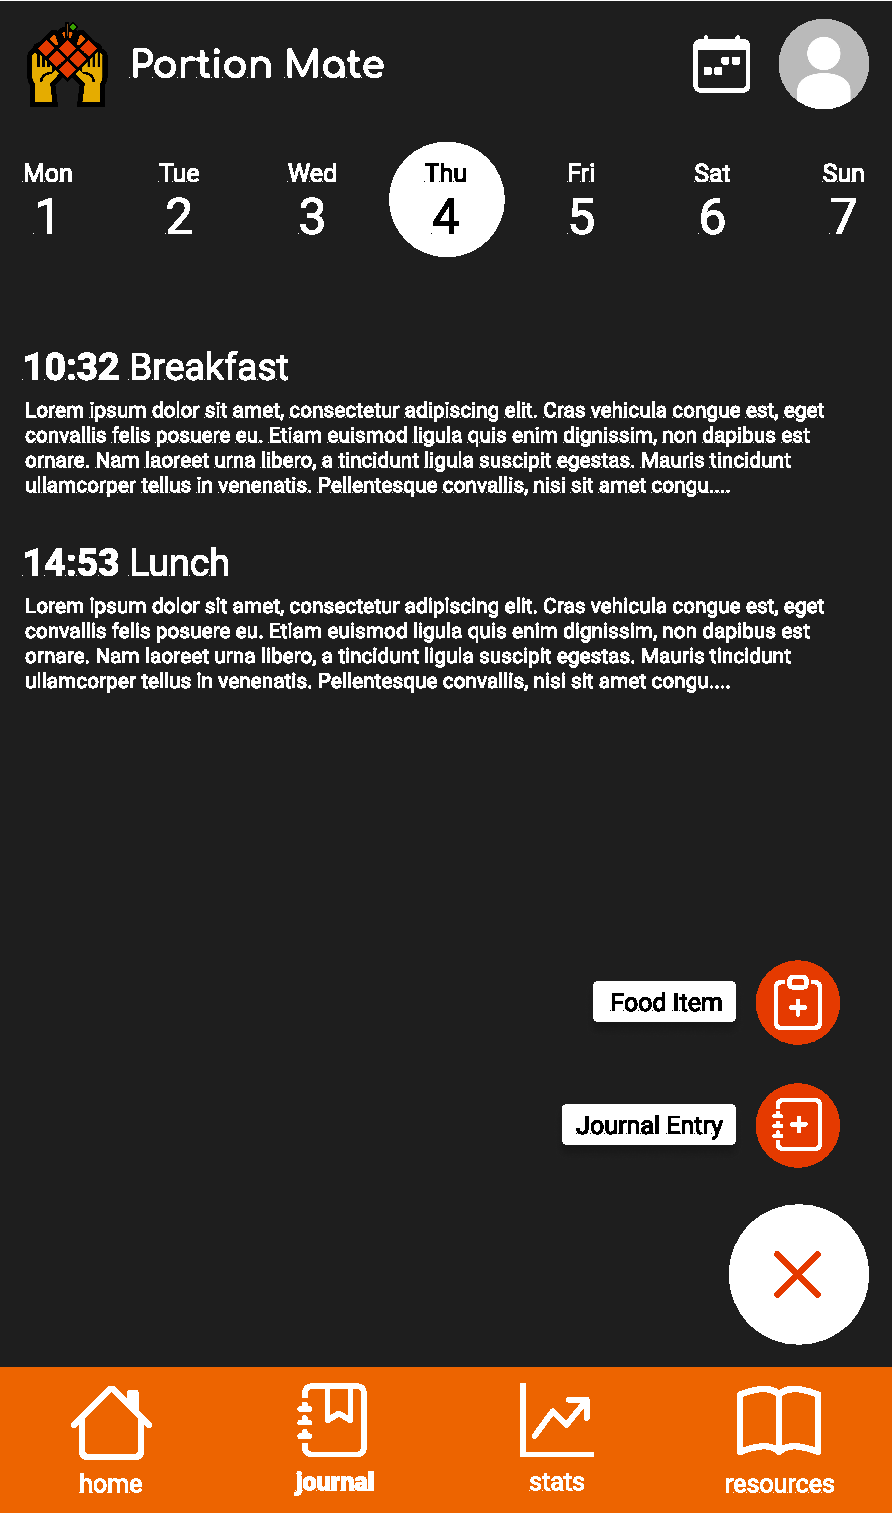
\includegraphics[height=5cm]{wireframes/Journal Action Button Menu [dark].pdf}}
    \caption{Journal (dark)}
    \end{subfigure}\hfill
    \begin{subfigure}{.24\textwidth}
    \centering
    \frame{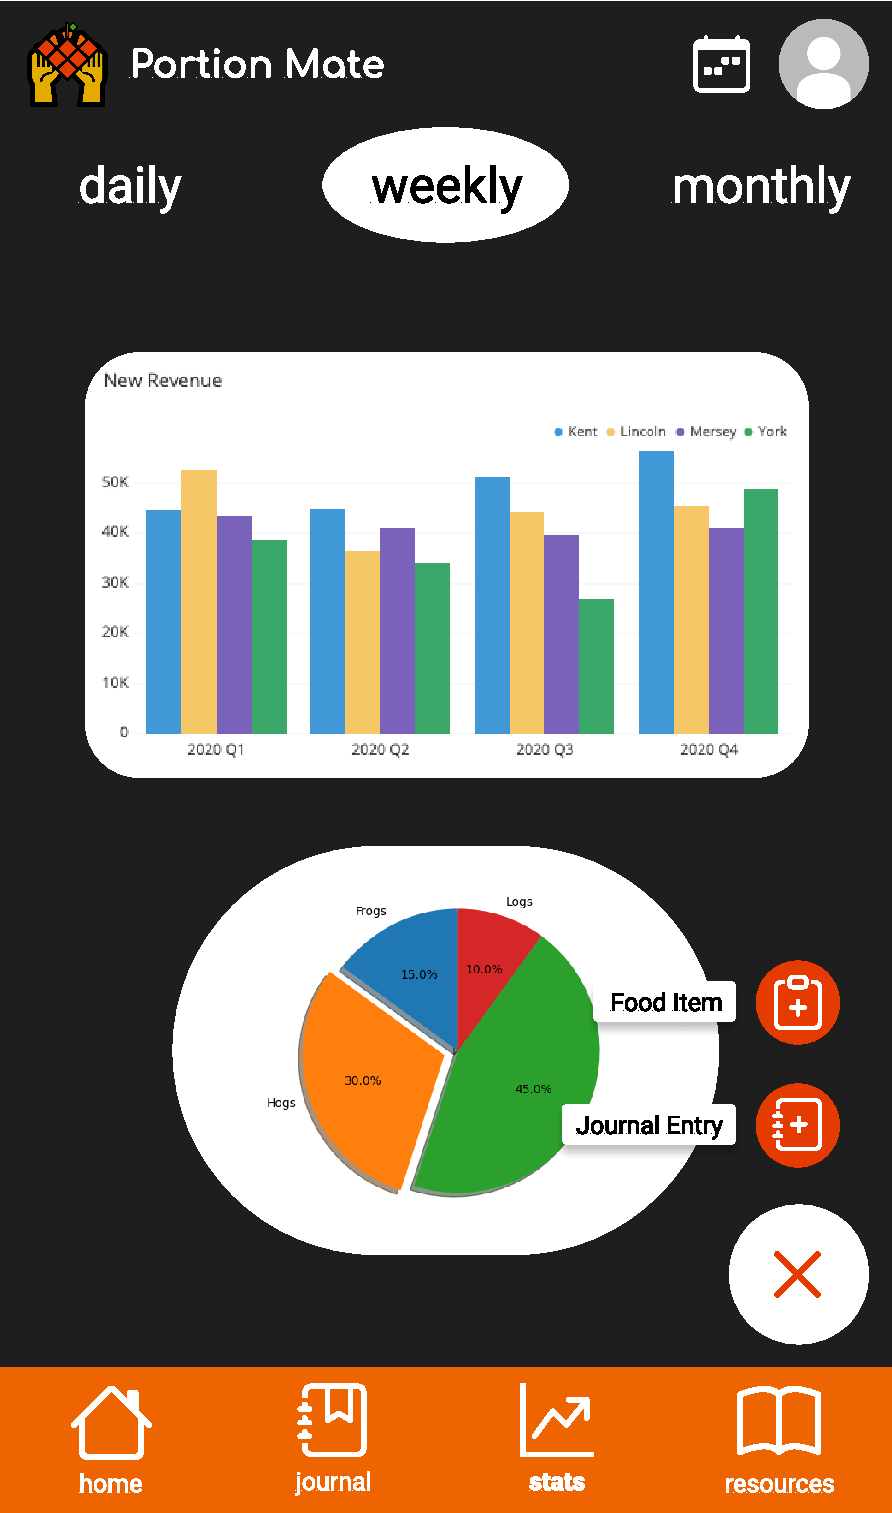
\includegraphics[height=5cm]{wireframes/Stats Action Button Menu [dark].pdf}}
    \caption{Stats (dark)}
    \end{subfigure}\hfill
    \begin{subfigure}{.24\textwidth}
    \centering
    \frame{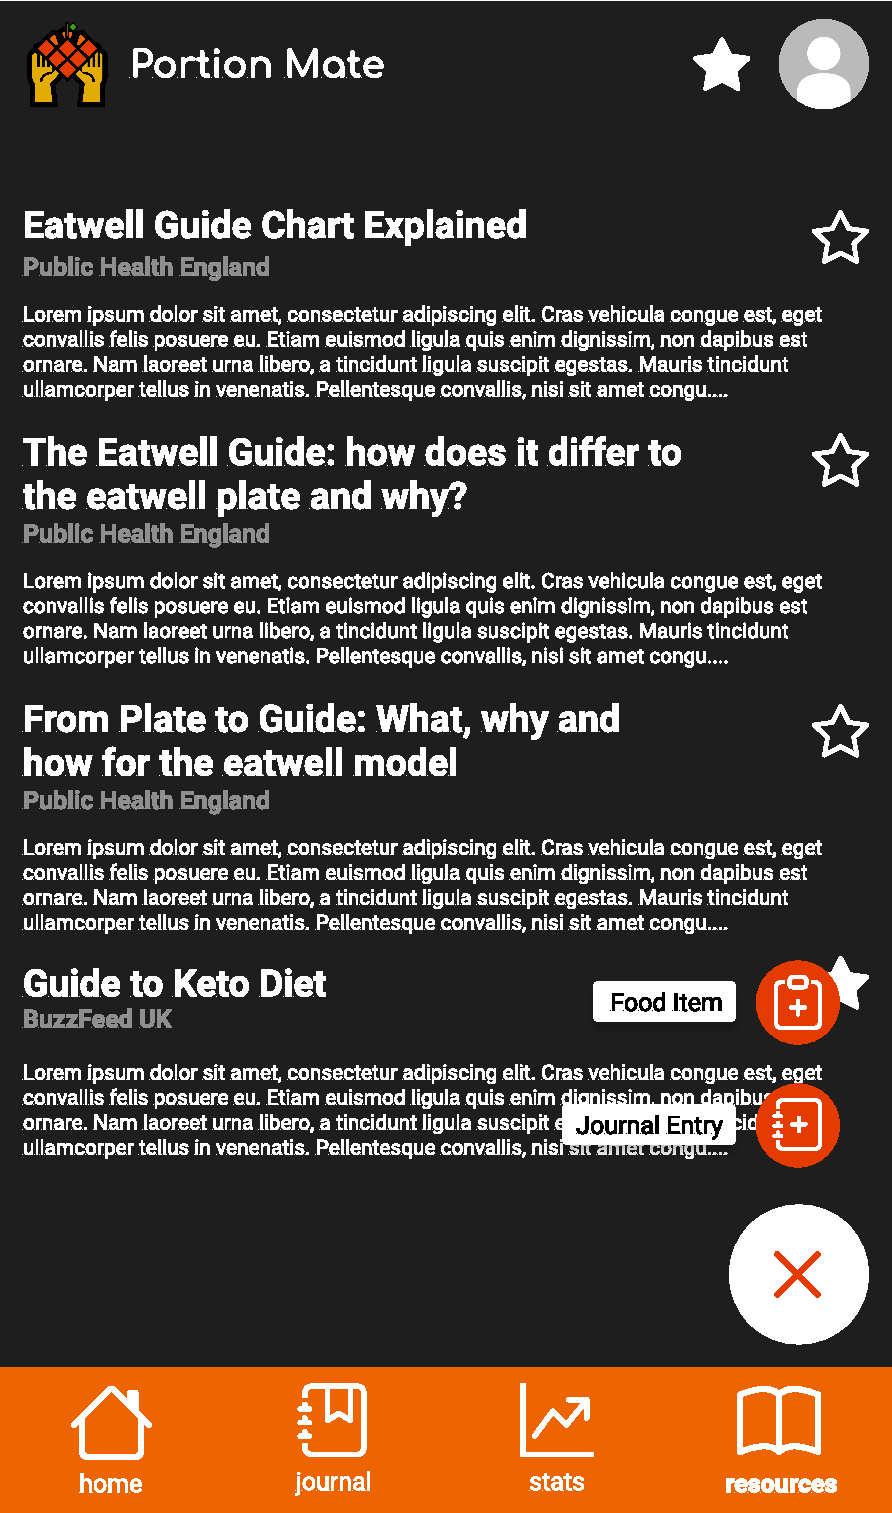
\includegraphics[height=5cm]{wireframes/Resources Action Button Menu [dark].pdf}}
    \caption{Resources (dark)}
    \end{subfigure}
    \caption{Floating Action Button preview on different screens (wireframes)}%\label{fig:wireframes_fab}
\end{figure}

\begin{figure}
    \centering
    \noindent\begin{subfigure}{.24\textwidth}
    \centering
    \frame{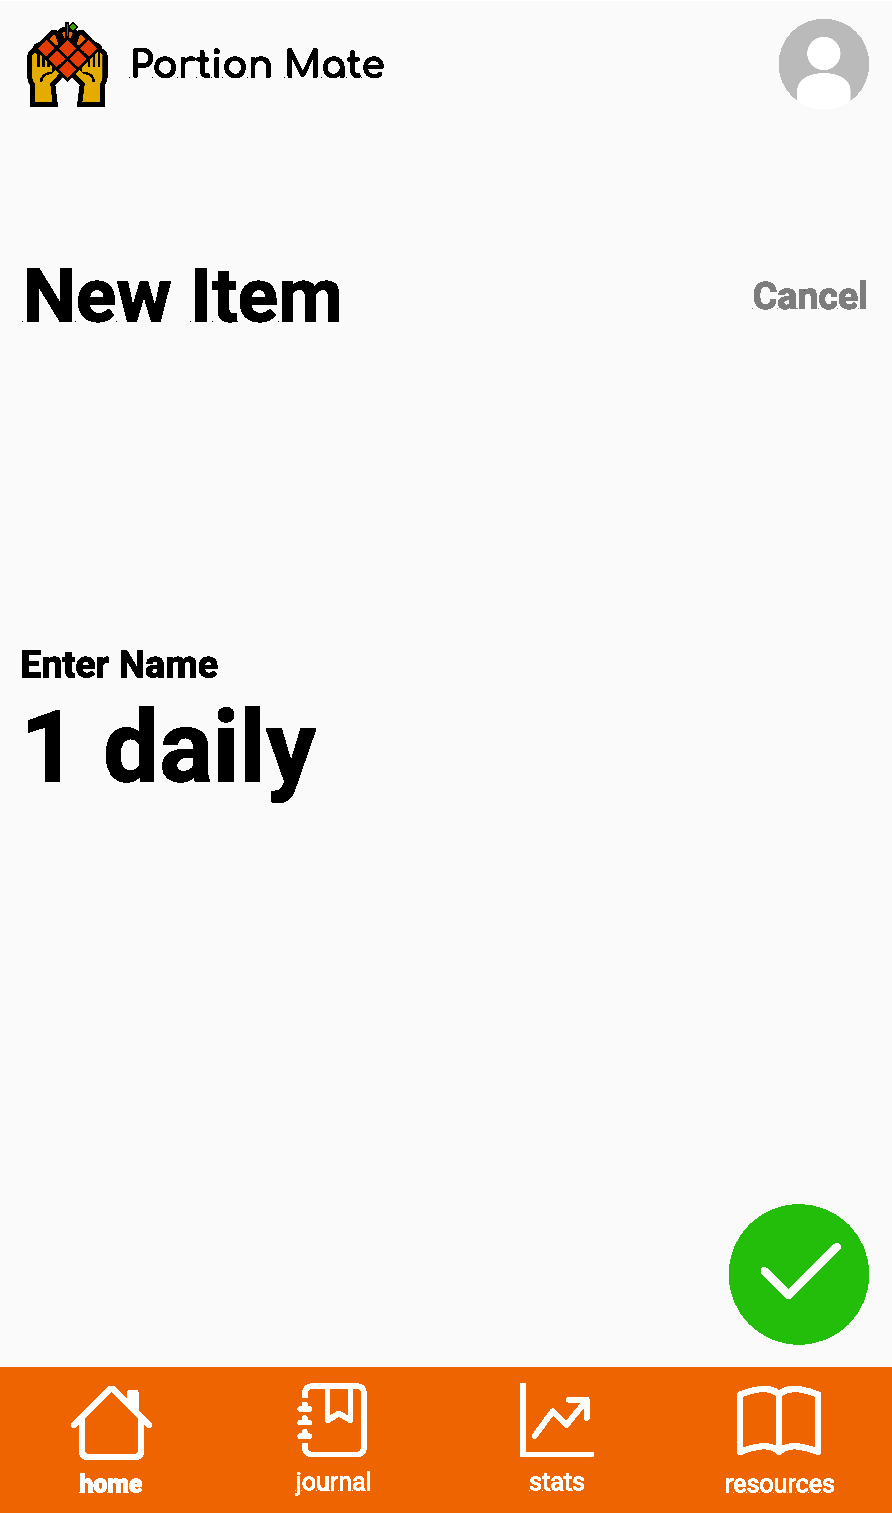
\includegraphics[height=5cm]{wireframes/New Item [light].pdf}}
    \caption{Add portion item (light)}
    \end{subfigure}\hfill
    \begin{subfigure}{.24\textwidth}
    \centering
    \frame{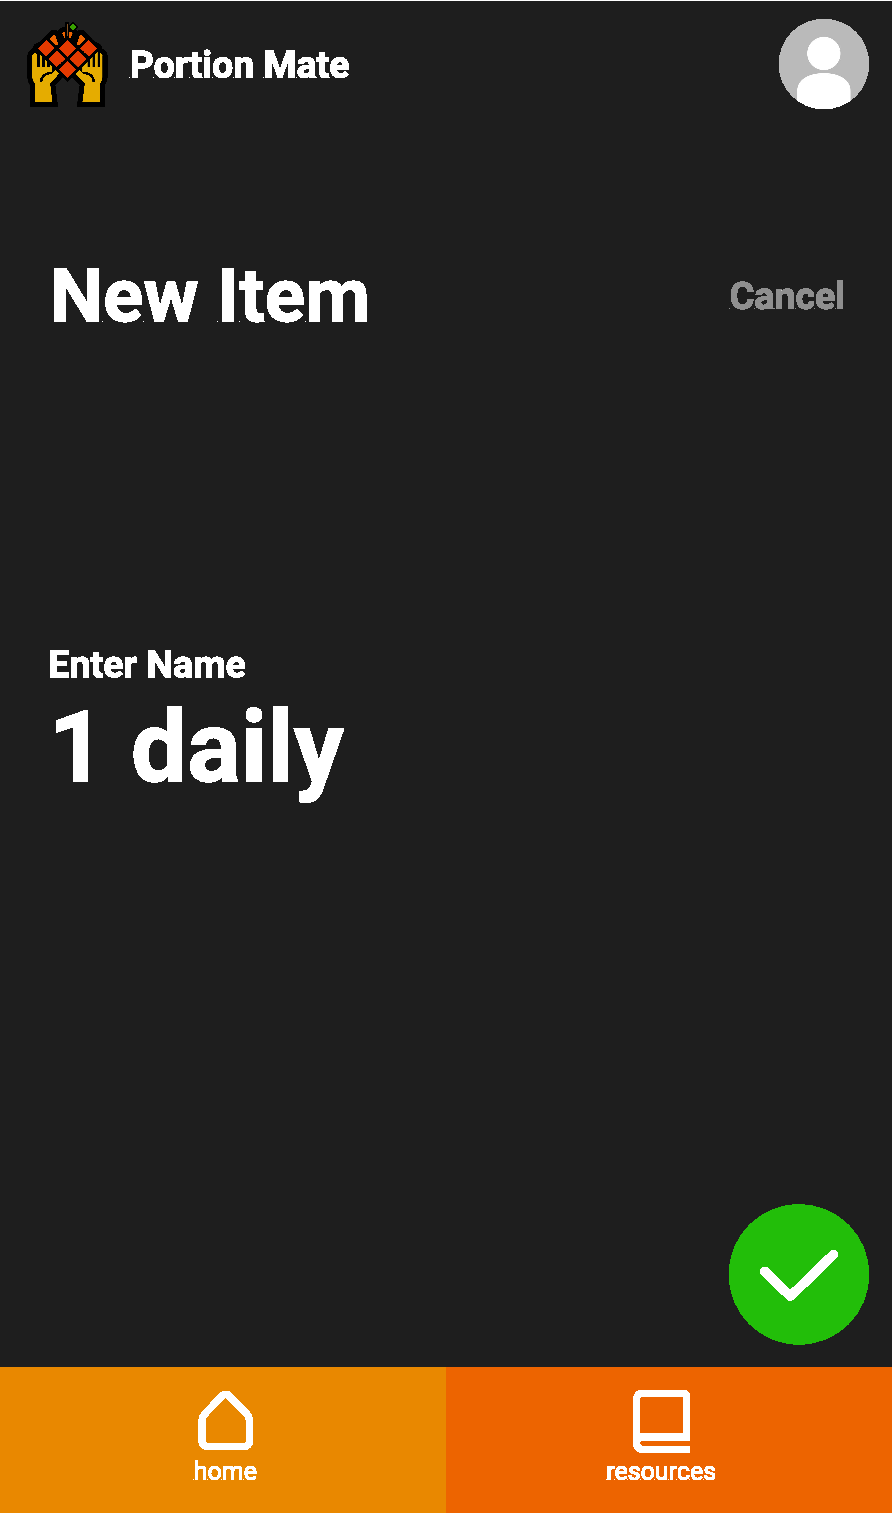
\includegraphics[height=5cm]{wireframes/New Item [dark].pdf}}
    \caption{Add portion item (dark)}
    \end{subfigure}\hfill
    \begin{subfigure}{.24\textwidth}
    \centering
    \frame{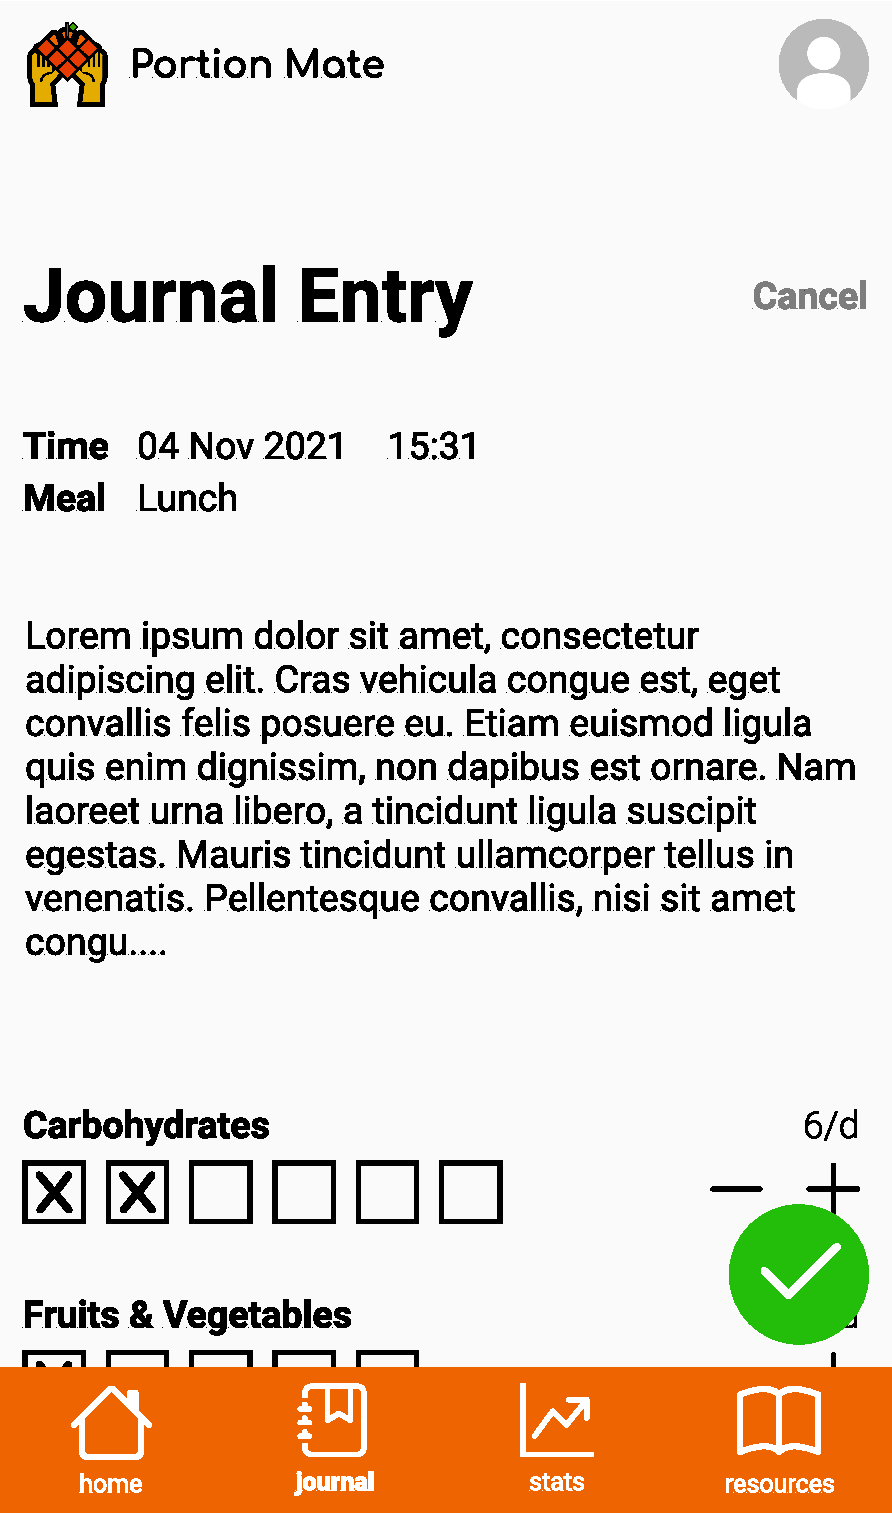
\includegraphics[height=5cm]{wireframes/New Entry [light].pdf}}
    \caption{Add diary entry (light)}
    \end{subfigure}\hfill
    \begin{subfigure}{.24\textwidth}
    \centering
    \frame{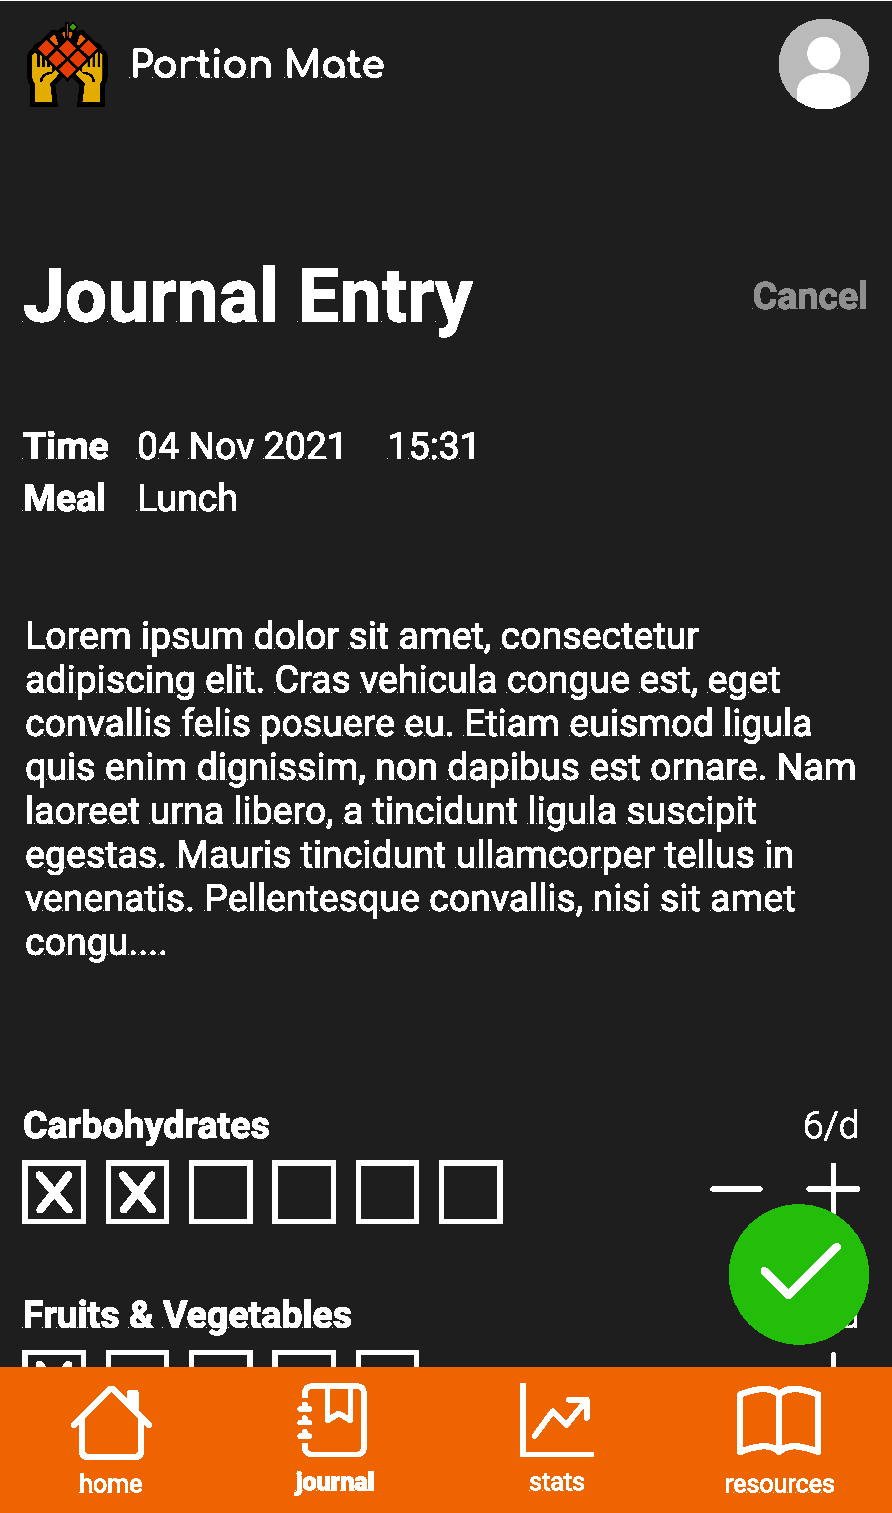
\includegraphics[height=5cm]{wireframes/New Entry [dark].pdf}}
    \caption{Add diary entry (dark)}
    \end{subfigure}
    \caption{Wireframes for adding logs and entries}%\label{fig:wireframes_for_entry}
\end{figure}

\begin{figure}
    \centering
    \noindent\begin{subfigure}{.24\textwidth}
    \centering
    \frame{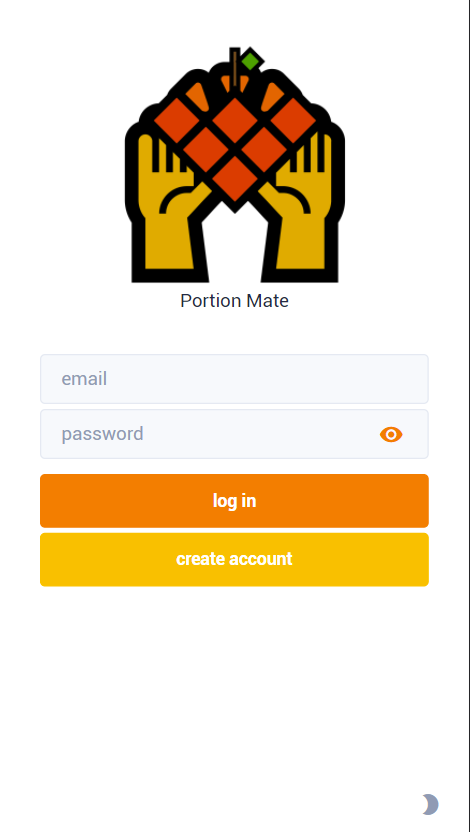
\includegraphics[height=5cm]{interface/Login Screen [light].png}}
    \caption{Login form (light)}
    \end{subfigure}\hfill
    \begin{subfigure}{.24\textwidth}
    \centering
    \frame{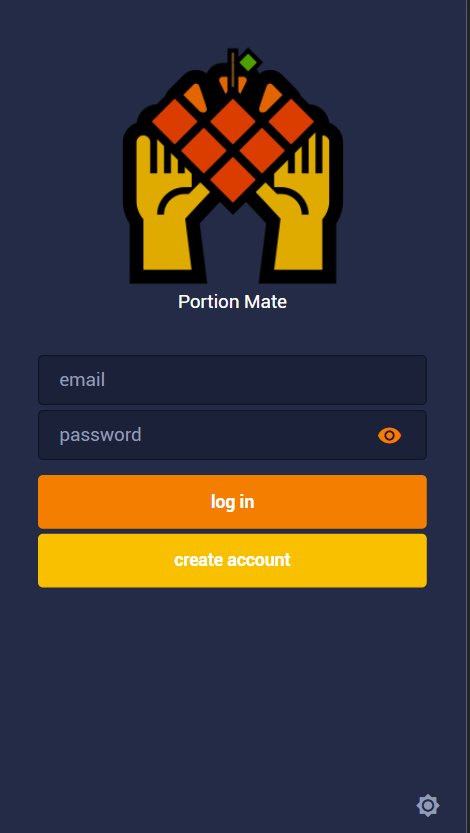
\includegraphics[height=5cm]{interface/Login Screen [dark].png}}
    \caption{Login form (dark)}
    \end{subfigure}\hfill
    \begin{subfigure}{.24\textwidth}
    \centering
    \frame{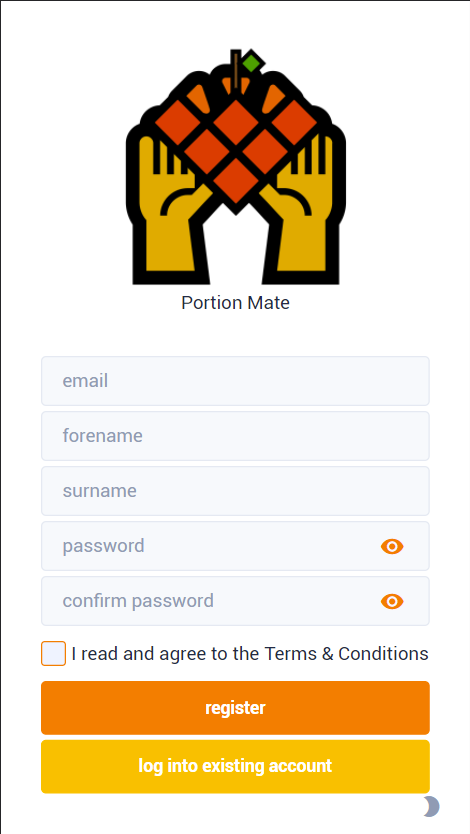
\includegraphics[height=5cm]{interface/Register Screen [light].png}}
    \caption{Register form (light)}
    \end{subfigure}\hfill
    \begin{subfigure}{.24\textwidth}
    \centering
    \frame{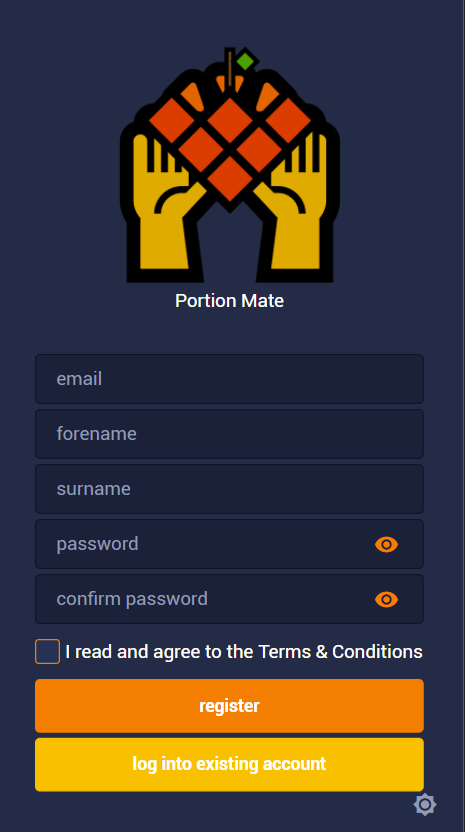
\includegraphics[height=5cm]{interface/Register Screen [dark].png}}
    \caption{Register form (dark)}
    \end{subfigure}
    \caption{Final interface for login and registration}
\end{figure}

\begin{figure}
    \centering
    \noindent\begin{subfigure}{.24\textwidth}
    \centering
    \frame{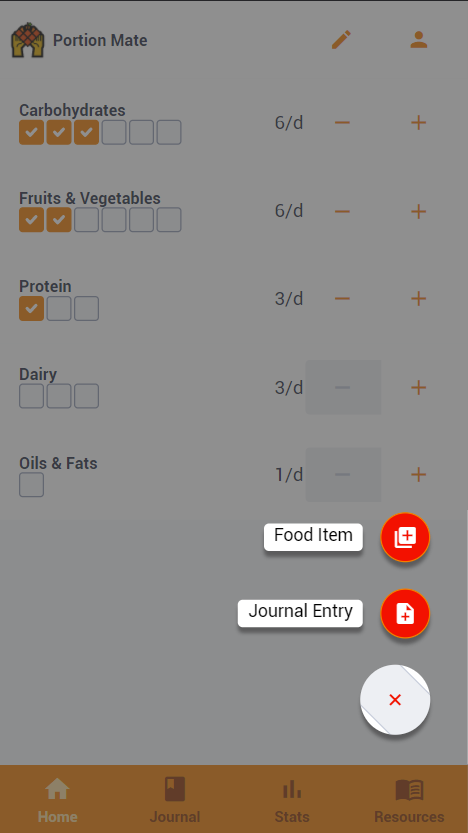
\includegraphics[height=5cm]{interface/Landing Action Button [light].png}}
    \caption{Home (light)}
    \end{subfigure}\hfill
    \begin{subfigure}{.24\textwidth}
    \centering
    \frame{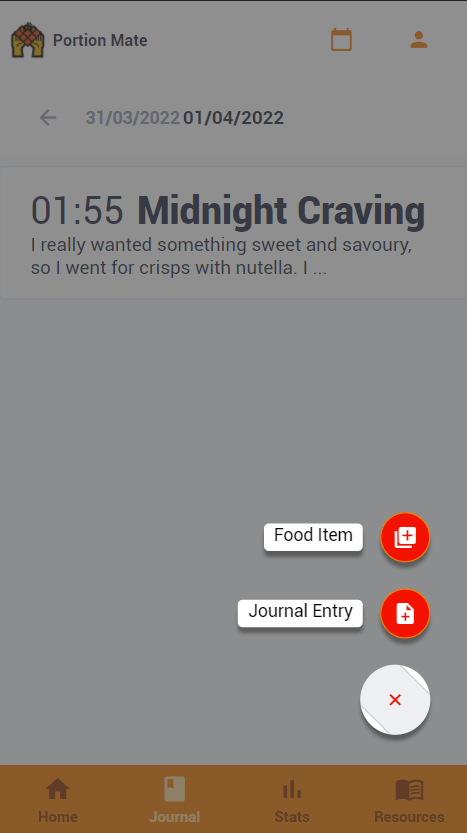
\includegraphics[height=5cm]{interface/Journal Action Button [light].png}}
    \caption{Journal (light)}
    \end{subfigure}\hfill
    \begin{subfigure}{.24\textwidth}
    \centering
    \frame{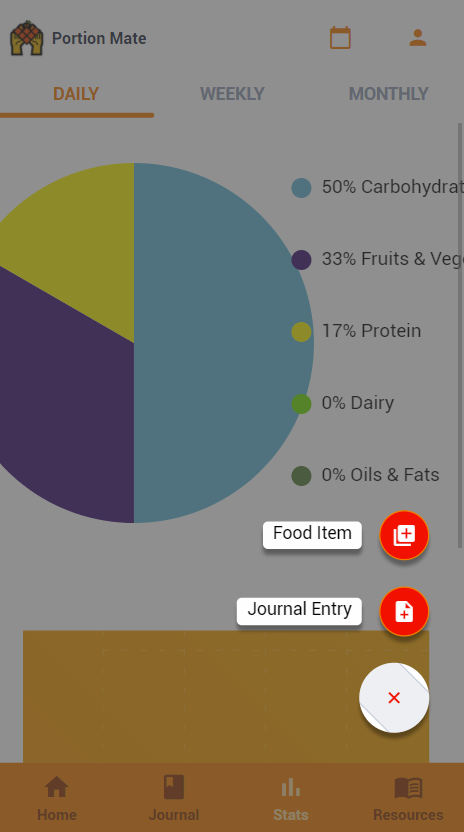
\includegraphics[height=5cm]{interface/Stats Action Button [light].png}}
    \caption{Stats (light)}
    \end{subfigure}\hfill
    \begin{subfigure}{.24\textwidth}
    \centering
    \frame{
\includegraphics[height=5cm]{interface/Resources Action Button [light].png}}
    \caption{Resources (light)}
    \end{subfigure}
    \vskip\baselineskip
    \noindent\begin{subfigure}{.24\textwidth}
    \centering
    \frame{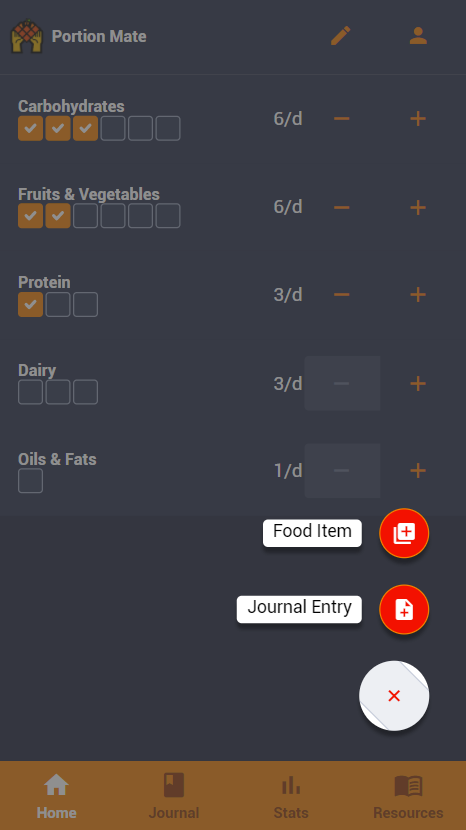
\includegraphics[height=5cm]{interface/Landing Action Button [dark].png}}
    \caption{Home (dark)}
    \end{subfigure}\hfill
    \begin{subfigure}{.24\textwidth}
    \centering
    \frame{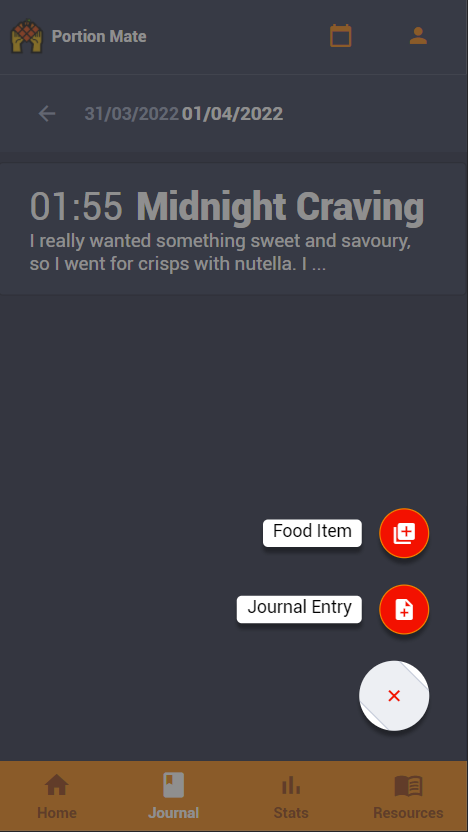
\includegraphics[height=5cm]{interface/Journal Action Button [dark].png}}
    \caption{Journal (dark)}
    \end{subfigure}\hfill
    \begin{subfigure}{.24\textwidth}
    \centering
    \frame{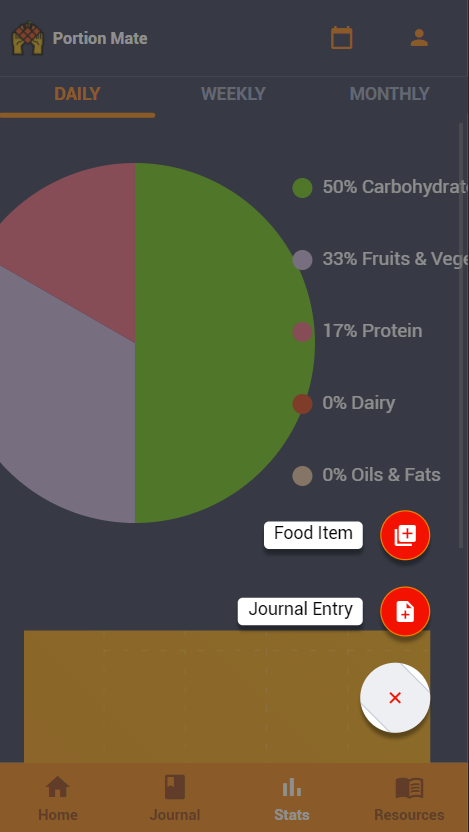
\includegraphics[height=5cm]{interface/Stats Action Button [dark].png}}
    \caption{Stats (dark)}
    \end{subfigure}\hfill
    \begin{subfigure}{.24\textwidth}
    \centering
    \frame{
\includegraphics[height=5cm]{interface/Resources Action Button [dark].png}}
    \caption{Resources (dark)}
    \end{subfigure}
    \caption{Floating Action Button preview on different screens (final)}%\label{fig:final_fab}
\end{figure}

\begin{figure}
    \centering
    \noindent\begin{subfigure}{.24\textwidth}
    \centering
    \frame{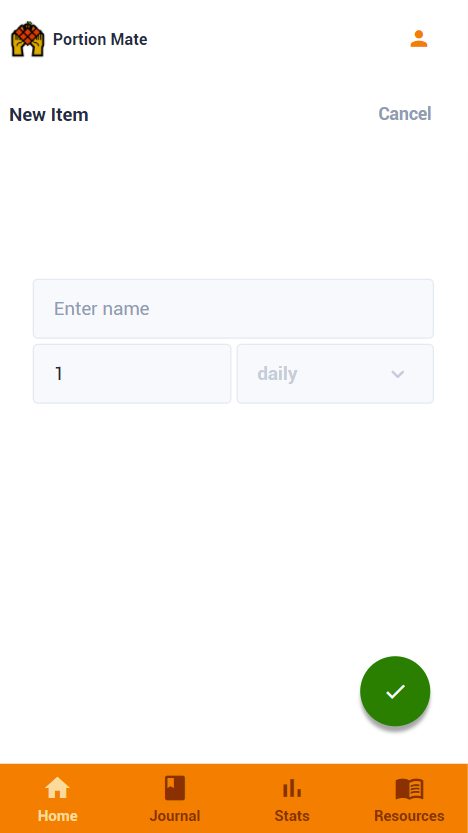
\includegraphics[height=5cm]{interface/New Item [light].png}}
    \caption{Add portion item (light)}
    \end{subfigure}\hfill
    \begin{subfigure}{.24\textwidth}
    \centering
    \frame{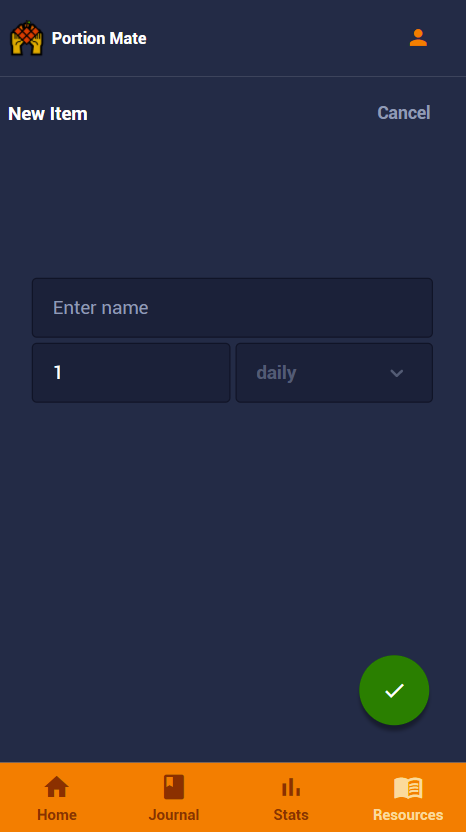
\includegraphics[height=5cm]{interface/New Item [dark].png}}
    \caption{Add portion item (dark)}
    \end{subfigure}\hfill
    \begin{subfigure}{.24\textwidth}
    \centering
    \frame{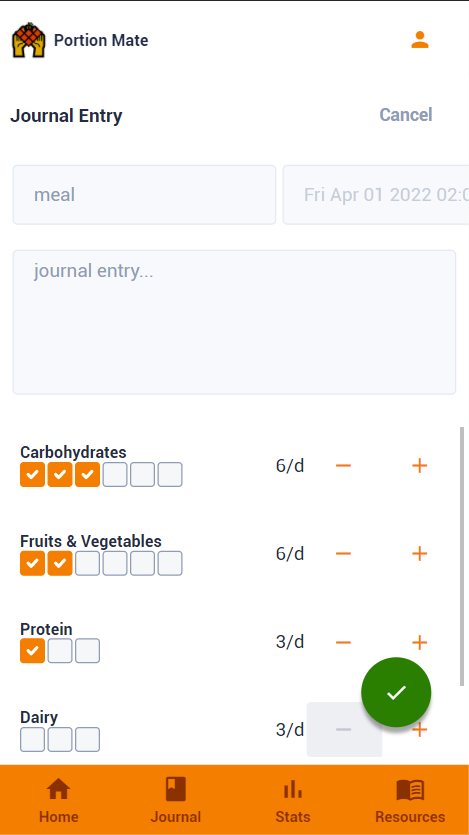
\includegraphics[height=5cm]{interface/New Entry [light].png}}
    \caption{Add diary entry (light)}
    \end{subfigure}\hfill
    \begin{subfigure}{.24\textwidth}
    \centering
    \frame{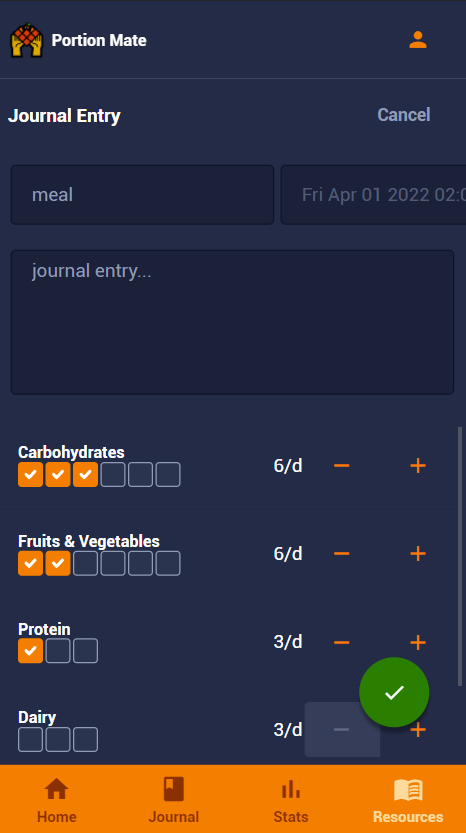
\includegraphics[height=5cm]{interface/New Entry [dark].png}}
    \caption{Add diary entry (dark)}
    \end{subfigure}
    \caption{Wireframes for adding logs and entries}%\label{fig:final_for_entry}
\end{figure}

\begin{table}
\centering
\setlength{\tabcolsep}{10pt}
\renewcommand{\arraystretch}{1.5}
\begin{tabular}{|l|llllllllll|}
\hline
                           & \textbf{P1}                                               & \textbf{P2}                        & \textbf{P3}                                               & \textbf{P4}                                               & \textbf{P5}                                               & \textbf{P6}                                               & \textbf{P7}                                               & \textbf{P8}                                               & \textbf{P9}                                               & \textbf{P10}                                              \\ \hline
\cellcolor[HTML]{EFEFEF}\textbf{S1}\textsuperscript{+} & \cellcolor[HTML]{680100}{\color[HTML]{FFFFFF} 1} & \cellcolor[HTML]{32CB00}4 & \cellcolor[HTML]{EFEFEF}3                        & \cellcolor[HTML]{34FF34}5                        & \cellcolor[HTML]{EFEFEF}3                        & \cellcolor[HTML]{EFEFEF}3                        & \cellcolor[HTML]{EFEFEF}3                        & \cellcolor[HTML]{34FF34}5                        & \cellcolor[HTML]{32CB00}4                        & \cellcolor[HTML]{FD6864}2                        \\
\textbf{S2}\textsuperscript{-}                         & 3                                                & 3                         & \cellcolor[HTML]{32CB00}4                        & \cellcolor[HTML]{680100}{\color[HTML]{FFFFFF} 1} & \cellcolor[HTML]{680100}{\color[HTML]{FFFFFF} 1} & \cellcolor[HTML]{680100}{\color[HTML]{FFFFFF} 1} & \cellcolor[HTML]{FD6864}2                        & \cellcolor[HTML]{680100}{\color[HTML]{FFFFFF} 1} & 3                                                & \cellcolor[HTML]{680100}{\color[HTML]{FFFFFF} 1} \\
\rowcolor[HTML]{34FF34} 
\cellcolor[HTML]{EFEFEF}\textbf{S3}\textsuperscript{+} & \cellcolor[HTML]{32CB00}4                        & \cellcolor[HTML]{32CB00}4 & \cellcolor[HTML]{EFEFEF}3                        & 5                                                & 5                                                & \cellcolor[HTML]{32CB00}4                        & 5                                                & 5                                                & 5                                                & 5                                                \\
\textbf{S4}\textsuperscript{-}                         & \cellcolor[HTML]{FD6864}2                        & 3                         & \cellcolor[HTML]{FD6864}2                        & \cellcolor[HTML]{680100}{\color[HTML]{FFFFFF} 1} & \cellcolor[HTML]{680100}{\color[HTML]{FFFFFF} 1} & \cellcolor[HTML]{FD6864}2                        & \cellcolor[HTML]{680100}{\color[HTML]{FFFFFF} 1} & \cellcolor[HTML]{680100}{\color[HTML]{FFFFFF} 1} & \cellcolor[HTML]{680100}{\color[HTML]{FFFFFF} 1} & \cellcolor[HTML]{680100}{\color[HTML]{FFFFFF} 1} \\
\cellcolor[HTML]{EFEFEF}\textbf{S5}\textsuperscript{+} & \cellcolor[HTML]{32CB00}4                        & \cellcolor[HTML]{32CB00}4 & \cellcolor[HTML]{EFEFEF}3                        & \cellcolor[HTML]{34FF34}5                        & \cellcolor[HTML]{34FF34}5                        & \cellcolor[HTML]{32CB00}4                        & \cellcolor[HTML]{34FF34}5                        & \cellcolor[HTML]{32CB00}4                        & \cellcolor[HTML]{34FF34}5                        & \cellcolor[HTML]{34FF34}5                        \\
\textbf{S6}\textsuperscript{-}                         & \cellcolor[HTML]{FD6864}2                        & \cellcolor[HTML]{32CB00}4 & \cellcolor[HTML]{FD6864}2                        & \cellcolor[HTML]{FD6864}2                        & \cellcolor[HTML]{680100}{\color[HTML]{FFFFFF} 1} & \cellcolor[HTML]{FD6864}2                        & \cellcolor[HTML]{680100}{\color[HTML]{FFFFFF} 1} & \cellcolor[HTML]{680100}{\color[HTML]{FFFFFF} 1} & \cellcolor[HTML]{680100}{\color[HTML]{FFFFFF} 1} & \cellcolor[HTML]{680100}{\color[HTML]{FFFFFF} 1} \\
\cellcolor[HTML]{EFEFEF}\textbf{S7}\textsuperscript{+} & \cellcolor[HTML]{32CB00}4                        & \cellcolor[HTML]{EFEFEF}3 & \cellcolor[HTML]{32CB00}4                        & \cellcolor[HTML]{32CB00}4                        & \cellcolor[HTML]{34FF34}5                        & \cellcolor[HTML]{32CB00}4                        & \cellcolor[HTML]{34FF34}5                        & \cellcolor[HTML]{34FF34}5                        & \cellcolor[HTML]{32CB00}4                        & \cellcolor[HTML]{34FF34}5                        \\
S8\textsuperscript{-}                         &                                                  &                           &                                                  &                                                  &                                                  &                                                  &                                                  &                                                  &                                                  &                                                  \\
\cellcolor[HTML]{EFEFEF}\textbf{S9}\textsuperscript{+} & \cellcolor[HTML]{EFEFEF}3                        & \cellcolor[HTML]{EFEFEF}3 & \cellcolor[HTML]{FD6864}2                        & \cellcolor[HTML]{34FF34}5                        & \cellcolor[HTML]{34FF34}5                        & \cellcolor[HTML]{32CB00}4                        & \cellcolor[HTML]{32CB00}4                        & \cellcolor[HTML]{34FF34}5                        & \cellcolor[HTML]{34FF34}5                        & \cellcolor[HTML]{34FF34}5                        \\
\textbf{S10}\textsuperscript{-}                        & \cellcolor[HTML]{FD6864}2                        & \cellcolor[HTML]{32CB00}4 & \cellcolor[HTML]{680100}{\color[HTML]{FFFFFF} 1} & \cellcolor[HTML]{680100}{\color[HTML]{FFFFFF} 1} & \cellcolor[HTML]{FD6864}2                        & \cellcolor[HTML]{FD6864}2                        & \cellcolor[HTML]{680100}{\color[HTML]{FFFFFF} 1} & \cellcolor[HTML]{680100}{\color[HTML]{FFFFFF} 1} & \cellcolor[HTML]{680100}{\color[HTML]{FFFFFF} 1} & \cellcolor[HTML]{680100}{\color[HTML]{FFFFFF} 1} \\ \hline
\end{tabular}
\caption{Participant responses for each statement}%\label{fig:participant_statement_map}
\end{table}

\begin{table}
\centering
\setlength{\tabcolsep}{10pt}
\renewcommand{\arraystretch}{1.5}
\begin{tabular}{|l|l|l|l|}
\hline
                      & \textbf{Score} & \textbf{Mean} & \textbf{SD} \\ \hline
\rowcolor[HTML]{EFEFEF} 
\textbf{Statement 1\textsuperscript{+}}  & 57.5           & 3.3           & 1.18        \\
\textbf{Statement 2\textsuperscript{-}}  & 75.0           & 2.0           & 1.09        \\
\rowcolor[HTML]{EFEFEF} 
\textbf{Statement 3\textsuperscript{+}}  & 87.5           & 4.5           & 0.67        \\
\textbf{Statement 4\textsuperscript{-}}  & 87.5           & 4.5           & 0.67        \\
\rowcolor[HTML]{EFEFEF} 
\textbf{Statement 5\textsuperscript{+}}  & 85.0           & 4.4           & 0.66        \\
\textbf{Statement 6\textsuperscript{-}}  & 82.5           & 1.7           & 0.90        \\
\rowcolor[HTML]{EFEFEF} 
\textbf{Statement 7\textsuperscript{+}}  & 82.5           & 4.3           & 0.64        \\
\textbf{\sout{Statement 8}\textsuperscript{-}}  &                &               &             \\
\rowcolor[HTML]{EFEFEF} 
\textbf{Statement 9\textsuperscript{+}}  & 77.5           & 4.1           & 1.04        \\
\textbf{Statement 10\textsuperscript{-}} & 85.0           & 1.6           & 0.91        \\ \hline
\end{tabular}
\caption{SUS Score, with mean and standard deviation, for each statement}%\label{fig:statement_stats}
\end{table}

\end{document}
